% -*- Mode:TeX -*-

%% The documentclass options along with the pagestyle can be used to generate
%% a technical report, a draft copy, or a regular thesis.  You may need to
%% re-specify the pagestyle after you \include  cover.tex.  For more
%% information, see the first few lines of mitthesis.cls. 

%\documentclass[12pt,vi,twoside]{mitthesis}
%%
%%  If you want your thesis copyright to you instead of MIT, use the
%%  ``vi'' option, as above.
%%
%\documentclass[12pt,twoside,leftblank]{mitthesis}
%%
%% If you want blank pages before new chapters to be labelled ``This
%% Page Intentionally Left Blank'', use the ``leftblank'' option, as
%% above. 

\documentclass[12pt,twoside]{mitthesis}
\usepackage{lgrind}
\pagestyle{plain}

%% in case I include .eps versions of all figures for those w/o pdftex
\usepackage{ifpdf}
\ifpdf
\usepackage[pdftex]{graphicx}
\else
\usepackage{graphicx}
\fi

\usepackage{amsmath,amssymb,amsfonts} % easily align arrays of equations
\usepackage{hyperref} % hyperlinks
\usepackage{subfig} % multi-part figures
\usepackage{pdfpages} % makes it easy to insert all those nsigmapi fits
\usepackage{multirow}
\usepackage{calrsfs} % fancier integrated luminosity script

% Feynman diagrams
\usepackage{feynmp}
\DeclareGraphicsRule{*}{mps}{*}{}

\begin{document}

% -*-latex-*-
% $Log: cover.tex,v $
% Revision 1.8  2008/05/13 15:02:15  jdreed
% Degree month is June, not May.  Added note about prevdegrees.
% Arthur Smith's title updated
%
% Revision 1.7  2001/02/08 18:53:16  boojum
% changed some \newpages to \cleardoublepages
%
% Revision 1.6  1999/10/21 14:49:31  boojum
% changed comment referring to documentstyle
%
% Revision 1.5  1999/10/21 14:39:04  boojum
% *** empty log message ***
%
% Revision 1.4  1997/04/18  17:54:10  othomas
% added page numbers on abstract and cover, and made 1 abstract
% page the default rather than 2.  (anne hunter tells me this
% is the new institute standard.)
%
% Revision 1.4  1997/04/18  17:54:10  othomas
% added page numbers on abstract and cover, and made 1 abstract
% page the default rather than 2.  (anne hunter tells me this
% is the new institute standard.)
%
% Revision 1.3  93/05/17  17:06:29  starflt
% Added acknowledgements section (suggested by tompalka)
% 
% Revision 1.2  92/04/22  13:13:13  epeisach
% Fixes for 1991 course 6 requirements
% Phrase "and to grant others the right to do so" has been added to 
% permission clause
% Second copy of abstract is not counted as separate pages so numbering works
% out
% 
% Revision 1.1  92/04/22  13:08:20  epeisach

% NOTE:
% These templates make an effort to conform to the MIT Thesis specifications,
% however the specifications can change.  We recommend that you verify the
% layout of your title page with your thesis advisor and/or the MIT 
% Libraries before printing your final copy.
\title{Longitudinal Double Spin Asymmetries of $\pi^{+/-}$ Production in $\vec{p}\vec{p}$ Collisions at 200 GeV}

\author{Adam Kocoloski}
% If you wish to list your previous degrees on the cover page, use the 
% previous degrees command:
%       \prevdegrees{A.A., Harvard University (1985)}
% You can use the \\ command to list multiple previous degrees
%       \prevdegrees{B.S., University of California (1978) \\
%                    S.M., Massachusetts Institute of Technology (1981)}
\prevdegrees{B.S. Physics, University of Dayton (2004) \\
             B.A. Philosophy, University of Dayton (2004)}
\department{Department of Physics}

% If the thesis is for two degrees simultaneously, list them both
% separated by \and like this:
% \degree{Doctor of Philosophy \and Master of Science}
\degree{Doctor of Philosophy}

% As of the 2007-08 academic year, valid degree months are September, 
% February, or June.  The default is June.
\degreemonth{June}
\degreeyear{2010}
\thesisdate{May 12, 2010}

%% By default, the thesis will be copyrighted to MIT.  If you need to copyright
%% the thesis to yourself, just specify the `vi' documentclass option.  If for
%% some reason you want to exactly specify the copyright notice text, you can
%% use the \copyrightnoticetext command.  
%\copyrightnoticetext{\copyright IBM, 1990.  Do not open till Xmas.}

% If there is more than one supervisor, use the \supervisor command
% once for each.
\supervisor{Bernd Surrow}{Associate Professor of Physics}

% This is the department committee chairman, not the thesis committee
% chairman.  You should replace this with your Department's Committee
% Chairman.
\chairman{Professor Thomas Greytak}{Associate Department Head for Education}

% Make the titlepage based on the above information.  If you need
% something special and can't use the standard form, you can specify
% the exact text of the titlepage yourself.  Put it in a titlepage
% environment and leave blank lines where you want vertical space.
% The spaces will be adjusted to fill the entire page.  The dotted
% lines for the signatures are made with the \signature command.
\maketitle

% The abstractpage environment sets up everything on the page except
% the text itself.  The title and other header material are put at the
% top of the page, and the supervisors are listed at the bottom.  A
% new page is begun both before and after.  Of course, an abstract may
% be more than one page itself.  If you need more control over the
% format of the page, you can use the abstract environment, which puts
% the word "Abstract" at the beginning and single spaces its text.

%% You can either \input (*not* \include) your abstract file, or you can put
%% the text of the abstract directly between the \begin{abstractpage} and
%% \end{abstractpage} commands.

% First copy: start a new page, and save the page number.
\cleardoublepage
% Uncomment the next line if you do NOT want a page number on your
% abstract and acknowledgments pages.
% \pagestyle{empty}
\setcounter{savepage}{\thepage}
\begin{abstractpage}
Spin dependent measurements provide incisive tests for modern theories of particle physics.  The discovery that the integral of the quark helicity distribution is much too small to account for the spin of the proton is an excellent case in point.  It inspired an intense period of theoretical scrutiny and a new generation of experiments to study \(\Delta g\), the helicity distribution of gluons in the nucleon.  In particular, the unique polarized proton collider at RHIC enables a class of asymmetry measurements that are directly sensitive to gluon polarization.

The STAR experiment at RHIC measures the double spin asymmetry \(A_{LL}\) for a variety of final states in collisions of longitudinally polarized protons in order to constrain \(\Delta g\). Asymmetries for mid-rapidity charged pion production benefit from large cross sections and the excellent tracking and particle identification capabilities of the STAR Time Projection Chamber. This thesis presents the first measurements of charged pion \(A_{LL}\) at STAR. The measurements are compared to predictions based on perturbative QCD calculations and from this comparison model-dependent constraints are placed on the integral gluon polarization \(\Delta G\).

\end{abstractpage}

% Additional copy: start a new page, and reset the page number.  This way,
% the second copy of the abstract is not counted as separate pages.
% Uncomment the next 6 lines if you need two copies of the abstract
% page.
% \setcounter{page}{\thesavepage}
% \begin{abstractpage}
% Spin dependent measurements provide incisive tests for modern theories of particle physics.  The discovery that the integral of the quark helicity distribution is much too small to account for the spin of the proton is an excellent case in point.  It inspired an intense period of theoretical scrutiny and a new generation of experiments to study \(\Delta g\), the helicity distribution of gluons in the nucleon.  In particular, the unique polarized proton collider at RHIC enables a class of asymmetry measurements that are directly sensitive to gluon polarization.

The STAR experiment at RHIC measures the double spin asymmetry \(A_{LL}\) for a variety of final states in collisions of longitudinally polarized protons in order to constrain \(\Delta g\). Asymmetries for mid-rapidity charged pion production benefit from large cross sections and the excellent tracking and particle identification capabilities of the STAR Time Projection Chamber. This thesis presents the first measurements of charged pion \(A_{LL}\) at STAR. The measurements are compared to predictions based on perturbative QCD calculations and from this comparison model-dependent constraints are placed on the integral gluon polarization \(\Delta G\).

% \end{abstractpage}

\cleardoublepage

\section*{Acknowledgments}

TBA

%%%%%%%%%%%%%%%%%%%%%%%%%%%%%%%%%%%%%%%%%%%%%%%%%%%%%%%%%%%%%%%%%%%%%%
% -*-latex-*-

\pagestyle{plain}
\include{contents}
\begin{fmffile}{feynman-diagrams}
\chapter{Theoretical Foundations}

\section{The Simple Parton Model}

Over the past century studies of spin in elementary particle physics have proven
their worth time and again, exposing weaknesses in theories that were otherwise
able to explain the measurements of the day. The first indication that the
proton was itself a composite particle came from a spin experiment, namely
Stern's discovery that the magnetic moment of the proton is incompatible with
the Dirac prediction for spin-\(\frac{1}{2}\) particles. As a result, the
\textit{structure function} was introduced in scattering cross sections to
codify our lack of knowledge about the true internal structure of the nucleon.

In 1964, Gell-Mann and Zweig independently proposed models
\cite{GellMann:1964nj, Zweig:1964jf} in which hadrons are composed of a set of
point-like elementary particles. These models provided a convenient taxonomy for
the zoo of particles which had been identified in experiments, but it was
unclear whether the ``quarks'', to use Gell-Mann's term, represented actual
physical entities. Five years later, Feynman and Bjorken and Paschos postulated
that the quarks -- they called them partons -- would behave quasi-free at high
energies \cite{Feynman:1969ej, Bjorken:1969ja}. A consequence of this model is
that in the high energy limit the structure functions of the proton measured in
deep inelastic scattering depend only on the (dimensionless) ratio of the
momentum transfer of the virtual photon and the energy loss of the scattered
electron. This ``Bjorken scaling'' behavior was soon observed at SLAC by
Friedman, Kendall, and Taylor \cite{Breidenbach:1969kd}. Physicists were
initially reluctant to identify the partons implied by the SLAC experiment with
the quarks in the models by Gell-Mann and Zweig, but eventually it became clear
that they were one and the same.

In the simple parton model Bjorken's $F_1$ structure function is expressed in
terms of the number densities $q(x)$ of quarks and $\bar q(x)$ of antiquarks
as
%
\begin{equation}
  F_1(x, Q^2) = \frac{1}{2}\sum_{j}{e_j^2[q_j(x) + \bar{q}_j(x)]}
\end{equation}
%
where the sum is taken over quark flavors $j$ and $e_j$ is the electromagnetic
charge of flavor $j$. In longitudinally polarized DIS we define an analogous
polarization density $\Delta q(x) \equiv q_+(x) - q_-(x)$ as the difference in
number density between quarks whose spins are aligned with the (longitudinal)
spin of the proton and quarks whose spins are anti-aligned; the polarized
analogue to $F_1$ is then
%
\begin{equation}
  g_1(x, Q^2) = \frac{1}{2}\sum_{j}{e_j^2[\Delta q_j(x) + \Delta \bar{q}_j(x)]}.
  \label{eqn:simple-g1}
\end{equation}

Typically one assumes \(SU(3)_F\) flavor symmetry and thus it is useful to
express the integral of \(g_1\) in terms of quantities which have specific
\(SU(3)_F\) transformation properties:
%
\begin{equation}
  \Gamma_1^p = \int_0^1 dx~g_1^p(x) = \frac{1}{9}\left[a_0 + \frac{3}{4}a_3 + \frac{1}{4}a_8\right].
  \label{eqn:g1}
\end{equation}
%
The \(a_j\) are the hadronic matrix elements of an octet of quark $SU(3)_F$
axial-vector currents $J_{5\mu}^i$ and a flavor singlet axial current
$J_{5\mu}^0$, and are related to the polarized quark densities in the proton as
%
\begin{eqnarray}
  a_0 & = & (\Delta u + \Delta \bar{u}) + (\Delta d + \Delta \bar{d}) + (\Delta s + \Delta \bar{s}) \nonumber \\
  a_3 & = & (\Delta u + \Delta \bar{u}) - (\Delta d + \Delta \bar{d}) \nonumber \\
  a_8 & = & (\Delta u + \Delta \bar{u}) + (\Delta d + \Delta \bar{d}) - 2(\Delta s + \Delta \bar{s})
  \label{eqn:su3-dis}
\end{eqnarray}
%
In the limit of massless partons the non-singlet currents are scale-independent quantities, and are known from $\beta$-decay measurements
\cite{Amsler:2008zzb}:
% Stiegler says a_8 = 3F+D, but Anselmino and Ashman agree on the (-)
\begin{eqnarray}
  a_3 & = & g_A = F+D = 1.2670 \pm 0.0035 \nonumber \\
  a_8 & = & 3F-D = 0.585 \pm 0.025.
  \label{eqn:beta-decay}
\end{eqnarray}
%
Hence a measurement of \(\Gamma_1^p\) allows the extraction of the flavor
singlet \(a_0\), the quark spin contribution to the spin of the proton. If one
assumes that the strange quark distribution does not contribute to the spin of
the proton, as Ellis and Jaffe did in 1974 \cite{Ellis:1973kp}, Equations
\ref{eqn:su3-dis} and \ref{eqn:beta-decay} allow a \textit{prediction} of the
quark spin contribution to the spin of the proton, namely \(a_0 = a_8 \approx
0.6\).

\section{First Experimental Tests}

In polarized deep inelastic scattering, a longitudinally polarized lepton beam
is scattered off of nucleon targets polarized parallel or perpendicular to the
beam axis. Asymmetries are formed by comparing event rates for scattering in
different spin configurations. For a spin $\frac{1}{2}$ target, the
asymmetries of interest are

% Stiegler 2.3 is useful here

\begin{equation}
  A_{\parallel} = \frac{\sigma^{\rightarrow \Leftarrow} - \sigma^{\rightarrow \Rightarrow}}{\sigma^{\rightarrow \Leftarrow} + \sigma^{\rightarrow \Rightarrow}}, ~~~~~~~
  A_{\perp} = \frac{\sigma^{\rightarrow \Uparrow} - \sigma^{\rightarrow \Downarrow}}{\sigma^{\rightarrow \Uparrow} + \sigma^{\rightarrow \Downarrow}}
\end{equation}

Spin-dependent cross sections can be calculated by contracting the elastic
Compton amplitude $T_{\mu \nu}$ with the photon polarization vectors; in the
presence of parity conservation and time reversal, four of these are
independent \cite{Close:1979bt}:
%
\begin{eqnarray}
  \sigma_{1/2} & = & F_1 + g_1 - \gamma^2 g_2, \nonumber \\
  \sigma_{3/2} & = & F_1 - g_1 + \gamma^2 g_2, \nonumber \\
  \sigma_L & = & -F_1 + F_2(1+\gamma^2)/(2x),  \nonumber \\
  \sigma_{TL} & = & \sqrt{2}\gamma (g_1+g_2).
\end{eqnarray}
%
Here $\gamma^2 = Q^2/v^2$. These four cross sections are commonly rearranged
into a pair of virtual photon asymmetries $A_1$ and $A_2$:
%
\begin{equation}
  A_1 = \frac{\sigma_{1/2} - \sigma_{3/2}}{\sigma_{1/2} + \sigma_{3/2}}, ~~~~ A_2 = \frac{\sigma_{TL}}{\sigma_T}
\end{equation}
%
The longitudinal and transverse DIS asymmetries can then be written in terms
of these virtual photon asymmetries. In the case of $A_{\parallel}$ we have
\begin{equation}
  A_{\parallel} = D(A_1 + \eta A_2),
\end{equation}
%
where the coefficients $D$ and $\eta$ can be approximated to first order in
$\gamma$ in terms of the usual DIS kinematic variables and $R =
\frac{\sigma_{L}}{\sigma_T}$:
% Detailed derivation of these results can be found in \cite{Anselmino:1994gn}
\begin{equation}
  D \approx \frac{y(2-y)}{y^2 + 2(1-y)(1+R)}, ~~~~~~~~ \eta \approx \frac{2(1-y)}{y(2-y)} \frac{\sqrt{Q^2}}{E}.
\end{equation}
%
Similar equations exist for $A_{\perp}$, such that a measurement of both
asymmetries allows an extraction of both $A_1$ and $A_2$. $D$ can be thought
of as a depolarization factor arising from the fact that the photon is not
fully aligned with the lepton beam, and $\eta$ is a kinematic factor that is
usually small. Finally, the polarized structure functions can be written in
terms of $A_{1,2}$:
\begin{equation}
  g_1 = \frac{F_2}{2x(1+R)}(A_1+\gamma A_2), ~~~~~ g_2 = \frac{F_2}{2x(1+R)}(A_2/\gamma - A_1).
\end{equation}
Thus, measurements of $A_{\parallel}$, $A_{\perp}$, $F_2$, and $R$ are
sufficient to determine the polarized structure functions of the nucleon.

The first DIS experiments to extract $g_1$ using this methodology were E80 and
E130, conducted in the late 1970s and early 1980s at SLAC. These experiments
scattered longitudinally polarized electron beams off of longitudinally
polarized proton targets and measured $A_{\parallel}^p$ in the range $0.1 < x <
0.7$. Using the positivity limit $A_2 < \sqrt{R}$ they determined that
$A_{\parallel}/D$ was a good approximation for $A_1$, and after exploiting that
assumption their results \cite{Alguard:1976bm, Baum:1983ha} were consistent with
expectations from the parton model.
% there are 2-3 more result papers cited in Baum:1983ha if I want them

In 1988, the European Muon Collaboration (EMC) published data on asymmetries of
longitudinally polarized muon beams scattering off of longitudinally polarized
proton targets. The EMC experiment boasted kinematic coverage down to $x =
0.01$, an order of magnitude lower than the earlier SLAC experiments, and the
Collaboration extracted measurements of the proton's $g_1$ structure function
using the same assumption that $A_1 \approx A_{\parallel}/D$. The EMC data on
$A_1$ are consistent with the results from SLAC in their overlapping kinematic
regime, but at low $x$ the EMC results deviate significantly from parton model
predictions. As shown in Figure \ref{fig:emc-g1p}, the value of $\Gamma_1^p$
obtained from the EMC extraction is incompatible with the prediction from Ellis
and Jaffe. Solving for the polarized parton densities using this result and the
beta decay measurements in \ref{eqn:beta-decay}, one finds that the strange
quarks possess a significant polarization antiparallel to the proton, and that
the quark spin contribution to the spin of the proton is only twelve percent:
%
% TODO these numbers come directly from EMC; should do it myself with my beta decay values
\begin{eqnarray}
  \langle S_z \rangle_{u} &=& \frac{1}{2}\left(\Delta u + \Delta \bar{u}\right) = 0.391 \pm 0.016 \pm 0.023, \nonumber \\
  \langle S_z \rangle_{d} &=& \frac{1}{2}\left(\Delta d + \Delta \bar{d}\right) = -0.236 \pm 0.016 \pm 0.023, \nonumber \\
  \langle S_z \rangle_{s} &=& \frac{1}{2}\left(\Delta s + \Delta \bar{s}\right) = -0.095 \pm 0.016 \pm 0.023, \nonumber \\
  \langle S_z \rangle_{quarks} &=& \frac{a_0}{2} = 0.060 \pm 0.047 \pm 0.069.
\end{eqnarray}
%
The EMC result sparked what was once termed a ``spin crisis'' in particle
physics. Successive polarized DIS experiments at CERN, SLAC, and DESY confirmed
and refined the EMC measurement of \(g_1^p\) with improved precision over a
wider kinematic range \cite{Adams:1994zd}, and measured both \(g_1^n\)
\cite{Anthony:1993uf} and \(g_1^d\) \cite{Adeva:1993km} which allowed a
verification of the critical Bjorken sum rule. Over the years the precise value
of \(\Gamma_1^p\) has shifted somewhat, but the implication remains the same ---
the na\"ive parton model cannot explain how the proton gets its spin.

\begin{figure}
  \includegraphics[width=1.0\textwidth]{figures/emc-g1p}
  \caption{EMC extraction of $g^1_p$ and its integral compared to the prediction from Ellis-Jaffe \cite{Ashman:1987hv}}
  \label{fig:emc-g1p}
\end{figure}

% discuss asympt. freedom, factorization, pdfs in "QCD and improved model"

% Then, in Access to DeltaG section, talk about scaling violation results and then pp asymmetries.

\section{QCD and the improved Parton Model}

The parton model results presented thus far assume that the photon scatters off
a free quark, a simplification which completely neglects the strong interaction.
In reality, quarks in the proton are tightly bound, constantly radiating and
reabsorbing gluons. Quantum chromodynamics (QCD) enhances the parton model with
interaction-dependent modifications of the simple parton model formulae. Two
effects are of particular interest in this work. The first is a violation of
parton density scaling; the distribution functions acquire a logarithmic
dependence on \(Q^2\) which is calculable in perturbative QCD. The second is an
anomalous gluonic contribution to \(a_0\), which at one time was thought to
offer a resolution to the ``spin crisis''. % TODO caveat about glossing over technical details, plus a citation of some review paper?

\subsection{Factorization and Scaling Violations}

\begin{figure}
  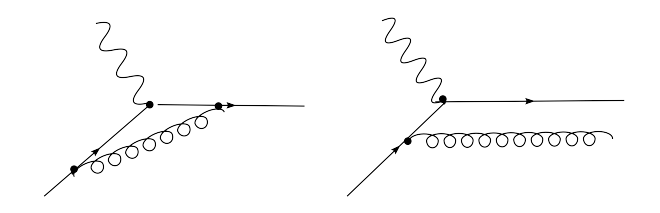
\includegraphics[width=1.0\textwidth]{figures/radiative-corrections}
  \caption{Examples of first-order radiative corrections to the quark-photon vertex.}
  \label{fig:radiative-corrections}
\end{figure}

Figure \ref{fig:radiative-corrections} illustrates two first-order gluonic
corrections to the quark-photon vertex. The diagrams contain collinear
divergences due to the massless quarks, so the size of each correction is
actually infinite. The standard technique for dealing with these infinities is
to factorize the reaction into a hard part calculable in perturbative QCD and a
soft part which must be parameterized from experimental observations. Generally
speaking, one encounters terms of the form
%
\begin{equation}
  \alpha_s~ln \frac{Q^2}{m_q^2} = \alpha_s~ln \frac{Q^2}{\mu^2} + \alpha_s~ln \frac{\mu^2}{m_q^2}.
\end{equation}
%
The first term on the right is included in the hard part of the interaction and
the second (infinite) term is absorbed into the parton distribution functions.
The factorization scale \(\mu^2\) is an arbitrary number, and exact physical
results cannot depend on it, but since perturbative results are never exact the
particular choice of scale is important. A common choice is
\(\mu^2 = Q^2\), which means that perfect Bjorken scaling of the distribution
functions is broken; that is \(q(x) \rightarrow q(x,Q^2)\). However, the
dependence on \(Q^2\) is only logarithmic and is calculable by a set of
evolution equations which are presented later.

QCD factorization is completely general and not limited only to higher-order
corrections to DIS. Consider the case of mid-rapidity pion production at a high
energy proton-proton collider. The factorization theorem allows one to write the
hadronic cross section for this process as a convolution of several independent
entities: PDFs describing the probability of picking out a given parton from
each proton, a hard partonic cross section, and a fragmentation function giving
the probability that an outgoing quark will fragment into a pion with a fraction
\(z\) of the parton's momentum. To wit:
%
\begin{equation}
  \sigma_{p_A+p_B \rightarrow \pi+X} = \sum_{a,b,c} f_a(x_A, Q^2) \otimes f_b(x_B, Q^2) \otimes \sigma_{a+b \rightarrow c + X} \otimes D_c^{\pi}(z)
  \label{eqn:factorization}
\end{equation}
%
The sum is over all parton flavors that contribute to the hadronic cross
section. The \(f_i\) are the parton distribution functions; \(D_c^{\pi}(z)\) is
the pion fragmentation function for quark flavor \(c\). The partonic cross
section is calculable using perturbative QCD when the \(Q^2\) of the interaction
is large, while the PDFs and FFs must be parameterized from experimental
results. Fortunately, those distribution functions are \textit{universal}; they
can be measured in any process (commonly \(e^+e^-\) collisions) and then applied
in the calculation of any other cross section. % TODO burton has a statement about the applicability of factorization in DIS and pp->jets with 2 references here

\subsection{Anomalous gluonic contribution to $\Gamma_1$}

A particularly interesting QCD correction to DIS is shown in Figure
\ref{fig:box-diagram}. This correction involves the gluonic version of the Adler
\cite{Adler:1969gk} and Bell and Jackiw \cite{Bell:1969ts} anomalous triangle
diagram, and results in a gluonic contribution to the flavor singlet matrix
element\footnote{This result is only valid in the \(AB\) and \(JET\)
renormalization schemes. In the \(\overline{MS}\) scheme, where \(\Delta
\Sigma\) itself varies with \(Q^2\), the gluonic contribution to \(a_0\) is
zero.}:
%
\begin{equation}
  a_0(Q^2) = \Delta \Sigma_q - 3\frac{\alpha_s(Q^2)}{2\pi} \Delta G(Q^2)
  \label{eqn:qcd-a0}
\end{equation}
%
This result invalidates the simple parton model formula \ref{eqn:su3-dis} for
\(a_0\) in terms of the quark spins. In the QCD enhanced parton model, a small
measured value of \(\Gamma_1^p\) (and thus a small \(a_0\)) does not necessarily
imply small quark polarization in the proton.

\begin{figure}
  \centering
  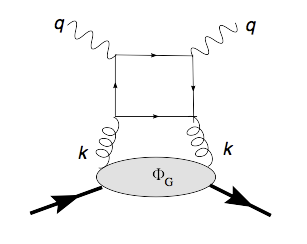
\includegraphics[width=0.5\textwidth]{figures/box-diagram}
  \caption{QCD diagram leading to the anomalous gluon contribution}
  \label{fig:box-diagram}
\end{figure}

\subsection{Spin Sum Rules}

The formulation in \ref{eqn:qcd-a0} has the attractive property that \(\Delta \Sigma_q\) is independent of \(Q^2\) and can be thought of as the quark helicity contribution even in the static (\(Q^2 \rightarrow 0\)) limit. Working in the light-cone gauge, one can write a sum rule for the proton spin which takes the form \cite{Hagler:1998kg, Harindranath:1998ve, Bashinsky:1998if}
%
\begin{equation}
  \frac{1}{2} = \frac{1}{2}\Delta \Sigma_q + \Delta G + L_q + L_g.
  \label{eqn:jaffe-sum-rule}
\end{equation}
%
Unfortunately, the last two terms are not experimentally accessible.  Lattice QCD can measure angular momentum contributions to the proton spin, but it does so in a different gauge and the sum rule \ref{eqn:jaffe-sum-rule} is not gauge invariant.

There exists an alternative sum rule \cite{Jaffe1990509, Ji:1996ek}
%
\begin{equation}
  \frac{1}{2} = \frac{1}{2}\Delta \Sigma_q + \hat{L}_q + \hat{J}_g
\end{equation}
%
where \(\hat{L}_q\) and \(\hat{J}_g\) correspond roughly to the orbital angular momentum of quarks and the total angular momentum of gluons in the nucleon. \(\hat{J}_q = \frac{1}{2}\Delta \Sigma + \hat{L}_q\) is measurable using deeply virtual Compton scattering, and \(\hat{J}_g\) can then in principle be obtained through the evolution of \(\hat{J}_q\).

The subtleties involved in decomposing the spin of the proton into experimental observables should not be viewed as a deterrent towards further experiments.  On the contrary, they are an opportunity for the data to lead the way to greater insight.


\section{Access to $\Delta G$}

The polarized gluon density affects a wide variety of observables,
and a rich experimental and computational program has developed over the past
few decades to strictly constrain it. The first experimental constraints on
\(\Delta G\) were obtained through measurements of the variation with \(Q^2\)
at fixed \(x\) of the \(g_1\) structure functions, while more recent
measurements in polarized DIS have focused on the photon-gluon fusion channel
that is directly sensitive to polarized glue. The results in this thesis rely
on a complementary and unique experimental program of polarized proton
collisions, where the partonic interactions frequently involve one or more
gluons in the initial state.

\subsection{Scaling Violations in parton densities}

QCD introduces a \(Q^2\) dependence into the parton distribution functions which is calculable using the evolution equations
%
\begin{eqnarray}
  \frac{d~\Delta q(x,Q^2)}{d~ln Q^2} &=& \frac{\alpha_s}{2 \pi} \left[ \Delta P_{qq} \otimes \Delta q + \Delta P_{qg} \otimes \Delta g \right], \nonumber \\
  \frac{d~\Delta g(x,Q^2)}{d~ln Q^2} &=& \frac{\alpha_s}{2 \pi} \left[ \Delta P_{gq} \otimes \Delta q + \Delta P_{gg} \otimes \Delta g \right].
\end{eqnarray}
%
The \(\Delta P\) are polarized splitting functions calculated perturbatively in \(\alpha_s\).  The original parton model equation for \(g_1\) \ref{eqn:simple-g1} becomes
%
\begin{equation}
  g_1(x, Q^2) = \frac{1}{2} \sum_{j} e_j^2 \left[\Delta q_j^2 + \Delta \bar{q}_j^2 + \frac{\alpha_s}{2 \pi} \left(\Delta C_j \otimes \left[\Delta q_j + \Delta \bar{q}_j\right] + \Delta C_g \otimes \Delta g\right)\right].
  \label{eqn:enhanced-g1}
\end{equation}
%
where the sum is over flavors and the \(\Delta C_j\) are Wilson coefficients. Given measurements of \(g_1\) at a fixed value of \(x\) and varying \(Q^2\), one can use \ref{eqn:enhanced-g1} to solve for the polarized gluon density. The  technique has proven very effective in unpolarized DIS, where a mix of fixed-target and collider data provides precise measurements of the structure functions across five decades in \(Q^2\) --- an excellent ``lever arm'' for the evolution equations.  In contrast, Figure \ref{fig:g1-versus-q2} plots the current world data on \(g_1\).  Extractions of \(\Delta g(x)\) from these fixed-target data are prone to significant uncertainties.  An example analysis from Leader, Sidorov, and Stamenov is shown in Figure \ref{fig:g1-deltag}; in that analysis, even the sign of the gluon polarization is not constrained by the data. The proposed Electron Ion Collider (EIC), a polarized analogue to HERA, would augment the current data on \(g_1\) with a broad range of high \(Q^2\) measurements and thus dramatically improve the constraints on polarized structure functions obtained through \(g_1\) evolution.

\begin{figure}
  \centering
  \includegraphics[width=0.7\textwidth]{figures/g1_x_q2}
  \caption{World data on the $g_1$ structure functions of the proton, plotted
  versus $Q^2$ for several values of $x$. An analysis of the variation with
  $Q^2$ yields a parameterization of the polarization gluon distribution.}
  % http://www2.lns.mit.edu/eic/Bruell.pdf
  \label{fig:g1-versus-q2}
\end{figure}

\begin{figure}
  \centering
  \includegraphics[width=0.6\textwidth]{figures/lss06_deltag}
  \caption{Extraction of the polarized gluon distribution from an analysis of
  scaling violations in DIS and SIDIS. The gray band indicates statistical and
  systematic uncertainties summed in quadrature. Analyses assuming positive,
  negative, and sign-changing gluon polarization all resulted in a comparable
  goodness-of-fit \cite{Leader:2006xc}}
  \label{fig:g1-deltag}
\end{figure}

\subsection{Photon-Gluon Fusion}

Given the relatively small lever arm in $Q^2$ currently available to constrain
$\Delta G$ via evolution of $g_1$, it is natural to pursue an alternative
approach involving observables that are directly linked to the gluon
polarization. In photon-gluon fusion (PGF), the lepton emits a real or virtual
photon that interacts with a gluon radiated from the nucleon to produce a
$q\bar{q}$ pair (see Figure \ref{fig:pgf}). PGF is a rare process compared to
scattering off of quarks in the nucleon, and as such analyses need a way to
enhance the signal to background ratio. The golden signature for PGF is charm
in the final state, since the nucleon itself has a negligible charm content.
Charm production has a small cross section, so analyses that look for
high-$p_T$ final states are also common.

Figure \ref{fig:pgf-deltag} summarizes results for the gluon polarization
extracted at leading order from analyses of photon-gluon fusion processes.
SMC, HERMES, and COMPASS have all released results based on the detection of
high-$p_T$ hadrons or jets, and COMPASS has released a single data point from
an analysis of charmed ($D^0$ and $D^*$) mesons. The data cover an $x$ range
of approximately $0.07 < \langle x \rangle < 0.2$ and restrict the magnitude
of the gluon polarization within that region. No NLO analysis of PGF data on
$\Delta G$ is currently available.

\begin{figure}
  \centering
  \begin{fmfgraph*}(200,150)
    \fmfleft{proton,gamma}
    \fmfright{proton',quark1,quark2}
    \fmf{fermion,width=2.5}{proton,v1}
    \fmf{fermion}{v1,proton'}
    \fmf{gluon}{v1,v2}
    \fmfblob{.15w}{v1}
    \fmf{fermion}{v2,quark1}
    \fmf{fermion}{v2,v3,quark2}
    \fmf{photon}{gamma,v3}

    % wow, it really feels like I should not have to do all of this
    \fmffixedx{0.}{v2,v3}
    \fmffixedy{0.}{v2,quark1}
    \fmffixedy{0.}{v3,quark2}
    \fmffixedy{0.}{v1,proton'}
    \fmffreeze
    \fmfshift{(0,-0.2h)}{v3}
    \fmfshift{(0.09w,-0.2h)}{quark2}
    \fmfshift{0,0.15h}{v1,proton'}
    
    % finally, add lines for outgoing quarks in struck proton
    \fmfi{plain}{vpath (__v1, __proton') shifted (thick*(-0.5,3.5))}
    \fmfi{plain}{vpath (__v1, __proton') shifted (thick*(-0.5,-3.5))}
  \end{fmfgraph*}
  \caption{Feynman diagram of photon-gluon fusion process}
  \label{fig:pgf}
\end{figure}


\begin{figure}
  \centering
  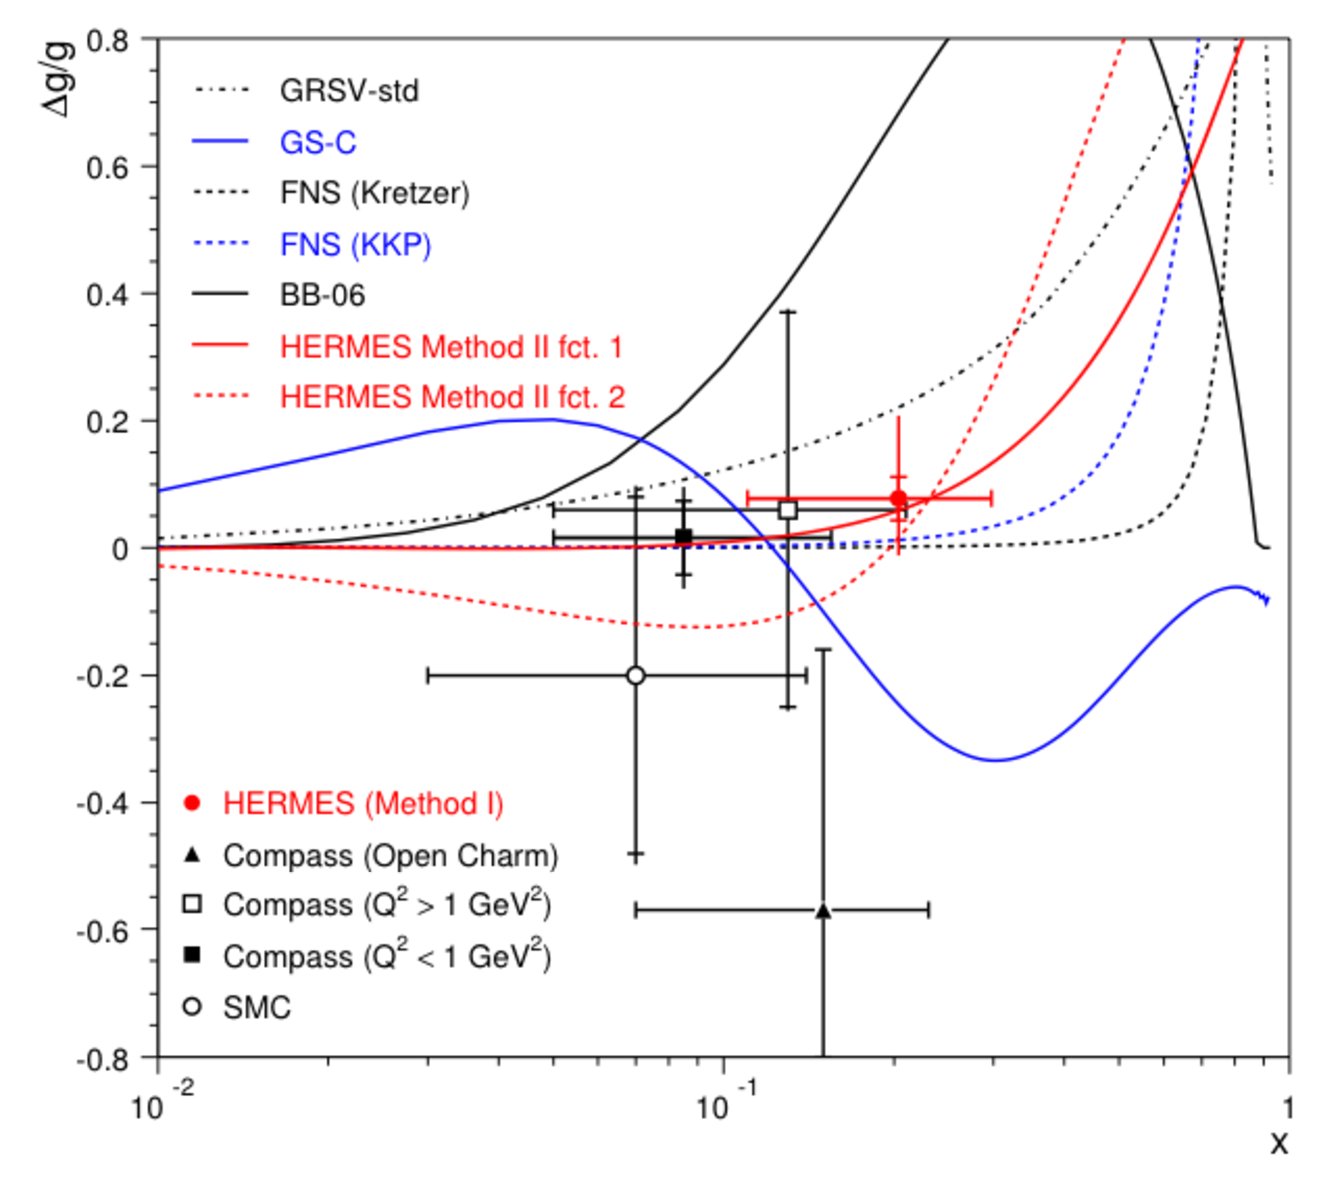
\includegraphics[width=0.7\textwidth]{figures/dgg-hermes-final}
  \caption{Compilation of $\Delta g(x)/g(x)$ measurements from SMC, HERMES,
  and COMPASS plotted versus momentum fraction \cite{Hasch:2009zza}.}
  \label{fig:pgf-deltag}
\end{figure}

% ... this is wrong, the number is just for the COMPASS open charm measurement, the most recent LO global analysis from COMPASS yields $\Delta g(x)/g(x) = -0.49~\pm~0.27~(stat)~\pm~0.11~(syst)$ at a scale $\mu^2 \sim 13~(GeV/c)^2$ and at an average gluon momentum fraction $\langle x \rangle ~\sim 0.11$ \cite{Alekseev:2009ey}.

%% Direct \Delta G figure without preliminary results
% \begin{figure}
%   \includegraphics[width=1.0\textwidth]{figures/compass_deltag}
%   \caption{\cite{Alekseev:2009ey}}
% \end{figure}

\subsection{Polarized Proton Collisions}

DIS is an electromagnetic process, so the techniques used to study the polarized gluon distribution in that environment must rely on higher-order QCD effects. In contrast, collisions of polarized protons are usually mediated by the strong force. Spin-dependent observables in these collisions are  directly sensitive to the polarized gluon content, as a significant fraction of hard scatterings contain one or more gluons in the initial partonic state. A given observable's particular sensitivity to polarized glue is calculable thanks to the triumvirate of asymptotic freedom, factorization, and PDF universality.  As of this writing, calculations performed at next-to-leading order (NLO) are the state of the art.

\begin{figure}\begin{center}
  \includegraphics[width=0.5\textwidth]{figures/partonic_asymmetry}
  \caption{Lowest-order analyzing powers for various partonic subprocesses
  present in polarized proton collisions \cite{Bunce:2000uv}.}
  \label{fig:partonic-asymmetries}
\end{center}\end{figure}

In principle one could directly measure a polarized cross section, e.g. a polarized analogue to \ref{eqn:factorization}.  In practice, a more precise result is obtained through asymmetry measurements that use the ratio of polarized and unpolarized cross sections to cancel out several sources of spin-independent uncertainty present in the absolute cross section measurements.  The observable of primary interest in this work is \(A_{LL}\), defined for inclusive pion production as
%
\begin{equation}
  A_{LL}(\pi + X) = \sum_{a,b,c} \frac{\Delta f_a(x_A, Q^2) \otimes \Delta f_b(x_B, Q^2) \otimes \left[ \hat{a}_{LL}^{ab \rightarrow cX} \sigma_{ab \rightarrow cX} \right] \otimes D_c^{\pi}(z)}{f_a(x_A, Q^2) \otimes f_b(x_B, Q^2) \otimes \sigma_{ab \rightarrow cX} \otimes D_c^{\pi}(z)}.
\end{equation}
%
\(\hat{a}_{LL}^{ab \rightarrow cX} \equiv \Delta \sigma_{ab \rightarrow cX} / \sigma_{ab \rightarrow cX}\) is the asymmetry of the underlying partonic hard scattering.  Figure \ref{fig:partonic-asymmetries} plots partonic asymmetries calculated using perturbative QCD for common subprocesses.  \(A_{LL}\) for charged pion production integrates over all five of these subprocess asymmetries.

\(A_{LL}\) can be measured and interpreted in a perturbative QCD context for a wide variety of final states. This thesis presents results on \(A_{LL}\) for inclusive charged pion production, as well as for charged pions produced azimuthally opposite an identified jet.  Figure \ref{fig:all-predictions} shows the effect of polarized glue on these observables.  The curves represent asymmetries calculated perturbatively at NLO assuming various polarized gluon distributions, ranging from an unpolarized glue (GRSV ZERO) to extreme fully-polarized scenarios (GRSV MIN).  The STD scenario in the GRSV \cite{Gluck:2000dy} set represented a best-fit extraction of polarized structure functions from \(g_1\) evolution data at the time of its release, while Gehrmann and Stirling's ``Set C'' \cite{Gehrmann:1995ag} is a scenario in which gluons are strongly polarized at low \(x\) but the overall integral of the gluon polarization is small thanks to a node in the distribution function.  Finally, the DSSV \cite{deFlorian:2008mr} set of structure functions is the first to incorporate data from measurements of \(A_{LL}\), specifically the inclusive \(\pi^0\) channel at PHENIX and the inclusive jet channel at STAR.  The measurements in this thesis can be included in a future update to the DSSV set and other similar global analyses in order to directly inform our understanding of the polarized gluon distribution.


\begin{figure}
  \subfloat{
    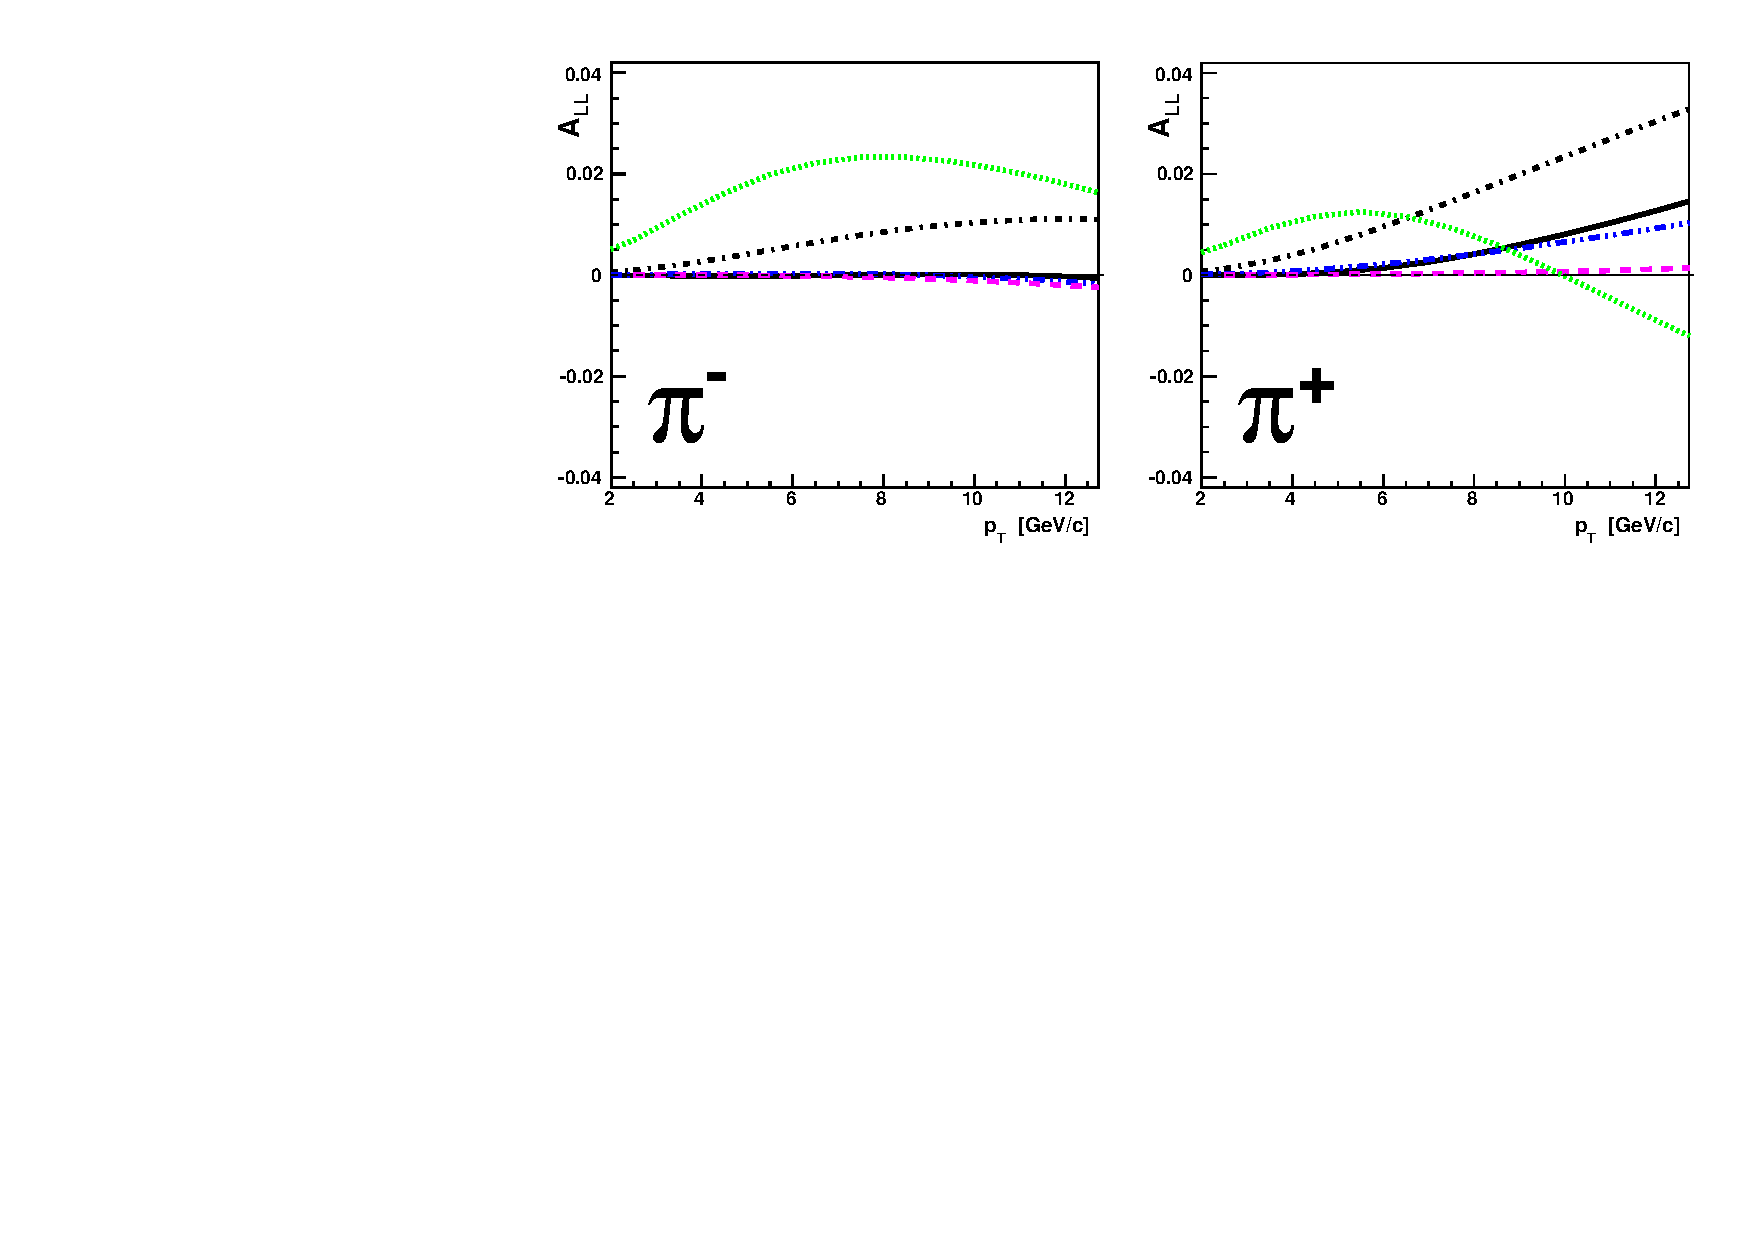
\includegraphics[width=1.0\textwidth]{figures/inclusive_predictions}
  }
  \newline
  \subfloat{
    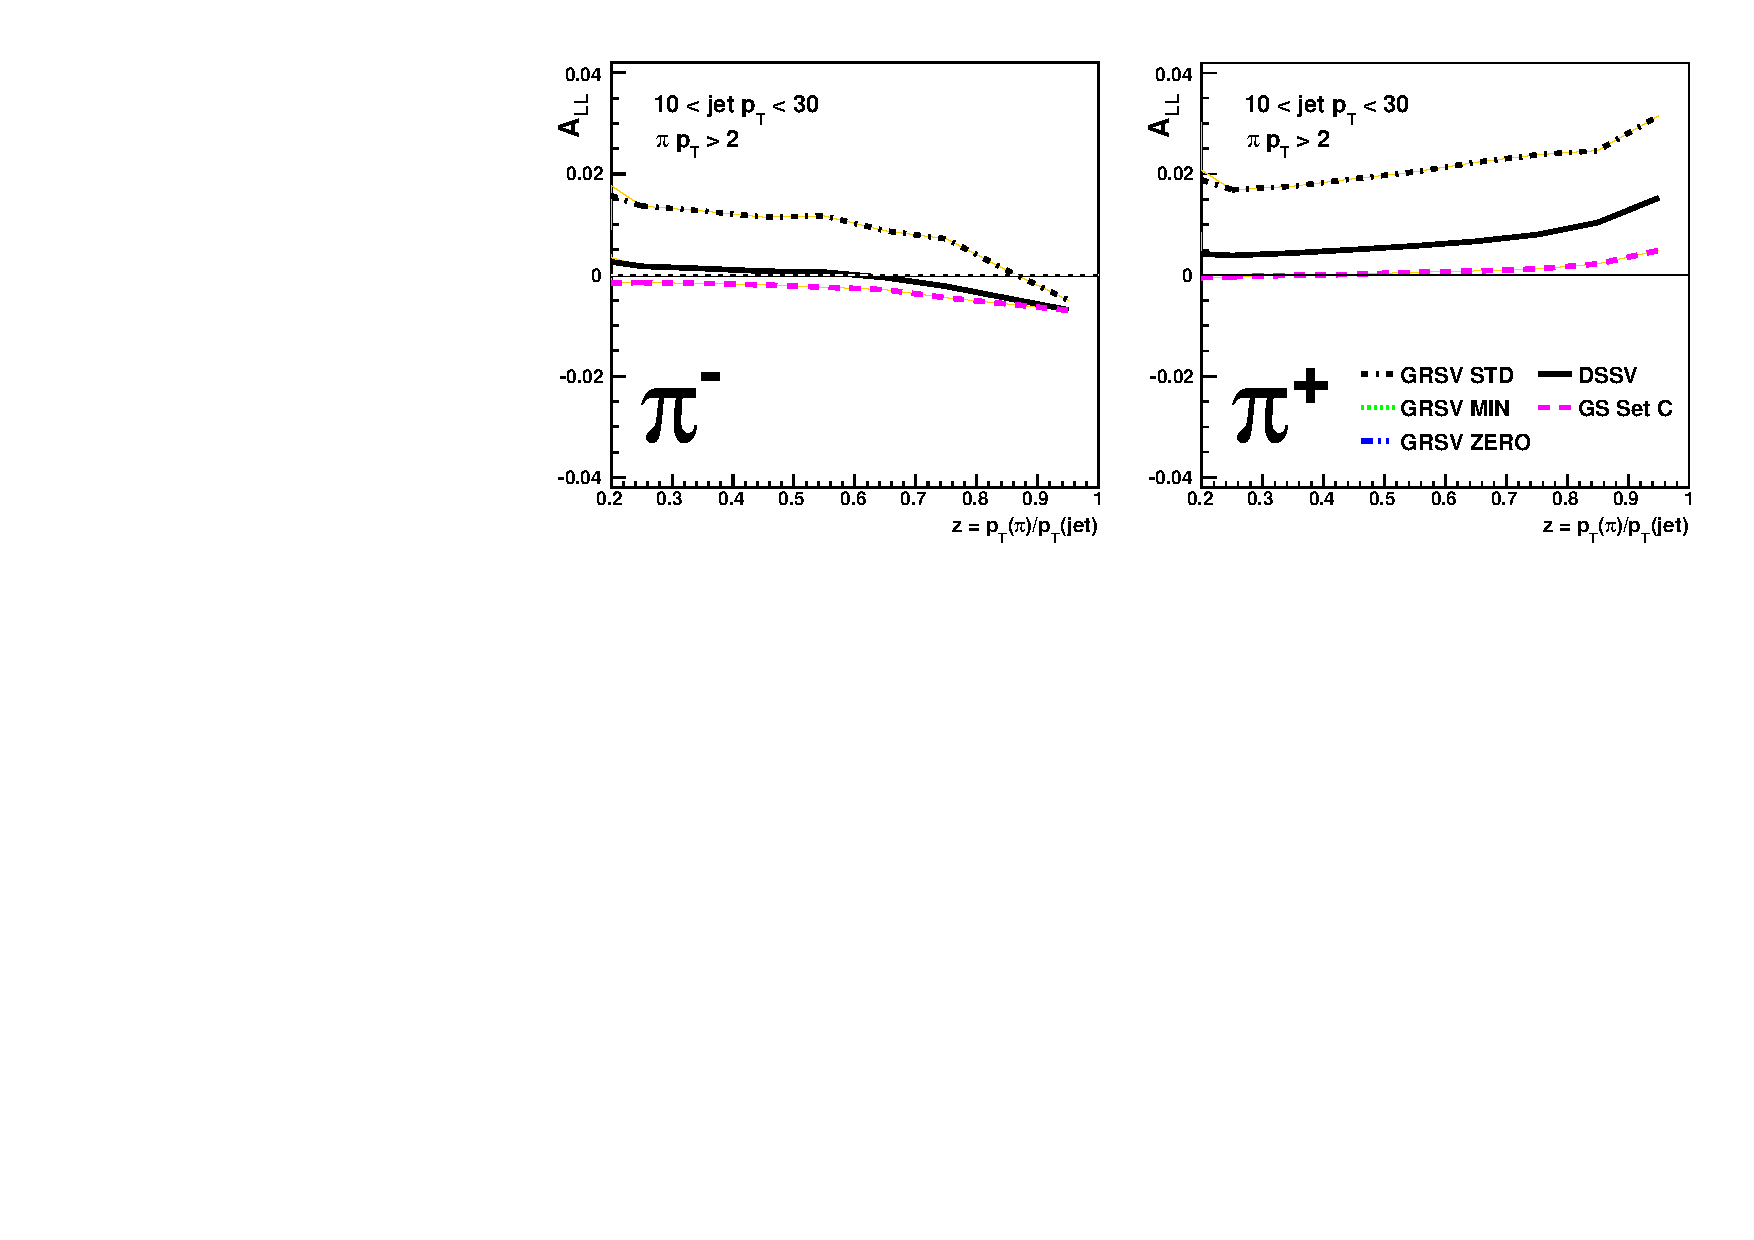
\includegraphics[width=1.0\textwidth]{figures/jet_pion_predictions}
  }
  \caption{Predictions for $A_{LL}$ assuming various input distributions for the gluon polarization \cite{Gluck:2000dy, Gehrmann:1995ag, deFlorian:2008mr}. The pion fragmentation functions can be found in \cite{deFlorian:2007nk}, and the NLO calculation was performed in the purely inclusive case by J\"ager et al. \cite{Jager:2002xm}, and in the jet + pion case by de Florian \cite{deFlorian:2009fw}.}
  \label{fig:all-predictions}
\end{figure}


\chapter{Experimental Facilities}

\section{The Relativistic Heavy Ion Collider (RHIC)}

\begin{figure}
  \begin{center}
    \includegraphics[width=0.8\textwidth]{figures/rhic-from-above}
  \end{center}
  \caption{The RHIC accelerator complex. Polarized protons are generated in
  OPPIS (not shown) and pass through the Linac, Booster, and AGS on their way
  to RHIC.}
  \label{fig:rhic}
\end{figure}

The Relativistic Heavy Ion Collider (RHIC) is an intersecting storage ring
located at Brookhaven National Laboratory in Upton, New York. Unusually
versatile for a collider, RHIC uses two independent superconducting rings to
collide beams of ions with mass numbers separately ranging from one to 197.
Recent beam configurations include protons on protons, deuterons on gold,
copper on copper, and gold on gold. Figure \ref{fig:rhic} shows a schematic
view of the RHIC accelerator complex. The main RHIC ring has a 3.8 kilometer
circumference and is comprised of six straight sections and six curved
sections. Collisions between the beams occur in the middle of each straight
section; four experimental halls are situated at the two (BRAHMS), six (STAR),
eight (PHENIX), and ten o'clock (PHOBOS) positions.

RHIC relies on a complex of smaller accelerators to prepare ion beams for
injection into the main ring. This work focuses on the systems used to
polarize and accelerate beams of protons, thus avoiding further discussion of
the Tandem Van de Graff generator used exclusively in heavy ion operations.
Polarized protons are produced using OPPIS \cite{Zelenski:2002gb,
Zelenski:2008zza}, an optically-pumped polarized ion source which typically
generates 0.5 mA, 400 $\mu$s pulses of ions, corresponding to
$\mathrm{9x10^{11}}$ ions per pulse. The pulsed nature of the beam is crucial
to achieving the RHIC design luminosity of
$\mathrm{2x10^{32}~cm^{-2}~s^{-1}}$. OPPIS polarizes protons by passing them
through a rubidium vapor pumped with circularly polarized laser light in a
strong magnetic field. The $\mathrm{H^+}$ ions pick up a polarized rubidium
electron through collisions in the vapor, and magnetic fields cause the
electron polarization to be transferred to the nucleus. Finally, the hydrogen
atoms are ionized to $\mathrm{H^-}$ when they pass through a sodium vapor.

The pulses of 35 keV $\mathrm{H^-}$ ions produced by OPPIS are accelerated by
the LINAC, Booster, and AGS on their way to RHIC. The LINAC strips off the
electrons and accelerates the protons to a kinetic energy of 200 MeV with an
efficiency of approximately 50\%. It injects the remaining $\sim
\mathrm{4x10^{11}}$ ions into the Booster ring in a single bunch. The Booster
accelerates the protons to 1.5 GeV and passes them on to the Alternating
Gradient Synchrotron (AGS), which accelerates them to the RHIC injection
energy of 25 GeV. RHIC propels the $\sim \mathrm{2x10^{11}}$ protons remaining
in each bunch to the desired collision energy, which can range from 30 GeV to
250 GeV. This work analyzes data collected with a beam energy of 100 GeV. More
details of the RHIC accelerator complex are available in references
\cite{Harrison:2003sb, Hahn:2003sc, Alekseev:2003sk}.

\subsection{Spin Dynamics and Siberian Snakes}

The evolution of the spin direction of a beam of polarized protons in external
magnetic fields is governed by the Thomas-BMT equation \cite{Thomas:1927yu,
Bargmann:1959gz},
%
\begin{equation}
  \frac{d\vec{P}}{dt} = -\left(\frac{e}{\gamma m}\right)[(G\gamma + 1) \vec{B}_{\perp} + (G + 1) \vec{B}_{\parallel}] \times \vec{P}.
\end{equation}
%
Comparing this equation with the Lorentz force equation governing the orbital
motion,
%
\begin{equation}
  \frac{d\vec{v}}{dt} = -\left(\frac{e}{\gamma m}\right)[\vec{B}_{\perp}] \times \vec{v},
\end{equation}
%
one realizes that, in a pure vertical magnetic field, the spin rotates
G$\gamma$ + 1 times faster than the orbital motion. This factor, referred to
as the spin tune $\nu_{sp}$, gives the number of full spin precessions for
every orbit.

An accelerating beam in a storage ring encounters depolarizing resonances
whenever the spin tune is equal to an integer multiple of the frequency with
which a spin-depolarizing magnetic field is encountered. In the simplest case,
a depolarizing field can be introduced by a magnet error or misalignment. For
these \textit{imperfection resonances}, the resonance condition is just
$G\gamma = n$. If $G\gamma$ is non-integral, the beam sees the depolarizing
field at a different point in its precession on each revolution, and the
effects tend to cancel out. The focusing fields themselves can also be a
source of depolarization; for these \textit{intrinsic resonances} the
resonance condition is $G\gamma = kP \pm \nu_y$, where $k$ is an integer,
$\nu_y$ is the vertical betatron tune, and $P$ is the superperiodicity.

The stable spin direction in an accelerating beam normally coincides with the
vertical magnetic field (longitudinal polarization at the interaction points
being achieved through the use of spin rotator magnets), but near a resonance
it is perturbed away from the vertical by the resonance driving fields. The
polarization loss when a beam is accelerated through one of these resonances
can be calculated analytically \cite{Froissart:1960zz}:
%
\begin{equation}
  \frac{P_f}{P_i} = 2 e^{-\pi |\epsilon|^2 / 2\alpha} -1.
\end{equation}
%
Here $\epsilon$ is the resonance strength and $\alpha$ is the change of the
spin tune per radian of the orbit angle. When the beam is slowly accelerated
($\alpha \ll |\epsilon|^2$) the stable spin direction changes adiabatically
and the result is a spin flip. In contrast, techniques such as a betatron tune
jump effectively result in $|\epsilon|^2 \ll \alpha$ and thus preserve the
polarization through the resonance. At high energies, the number and strength
of the resonances encountered make these traditional techniques impractical.
Instead, the RHIC rings employ ``Siberian Snake'' magnets
\cite{Derbenev:1978hv} which generate a 180\degree spin rotation about a
horizontal axis when the beam passes through them. In effect, the Siberian
Snakes ensure that the spin tune is an energy-independent half-integer, thus
avoiding all imperfection resonances as well as intrinsic resonances with an
appropriate choice of the betatron tune. RHIC is designed to achieve 70\%
polarization; the datasets analyzed in this work were taken with 45\% - 55\%
polarized beams, as certain elements of the accelerator complex (notably, a
Siberian Snake in the AGS) were still being commissioned.

\subsection{Polarimetry Systems\label{sec:polarimeters}}

RHIC polarimetry relies on the observation of small angle elastic scattering
in the Coulomb-Nuclear Interference (CNI) region. Two complementary varieties
of target are used: a thin carbon ribbon \cite{Jinnouchi:2004up} and a
hydrogen gas jet (H-Jet) \cite{Zelenski:2005mz, Okada:2006dd}. The carbon
ribbon boasts a large scattering cross section which allows a statistically
precise measurement of the beam polarization in a few seconds, but the
theoretical prediction for the analyzing power of this measurement includes an
unknown contribution from a hadronic spin flip amplitude. In contrast, the
hydrogen gas jet has a well-understood analyzing power but a much smaller
scattering cross section. The natural solution, then, is to calibrate the
results of the p+C CNI polarimeters with a measurement from the H-jet
polarimeter.

The p+C polarization measurements are performed using individual carbon ribbon
targets in each beam that are a mere 150 $\mathrm{\mathring{A}}$ thick.
Scatterings occur at a momentum transfer of 0.002 - 0.010 $\mathrm{GeV}^2$,
resulting in a small forward scattering angle for the proton and a recoil
carbon nucleus with less than 1 MeV of kinetic energy. Detection of the
scattered proton is not possible without drastic changes to the beam profile
at the polarimeter location, but the thinness of the target allows the recoil
nucleus to escape the target and reach one of a set of silicon strip detectors
arranged around it. The use of a thin target also allows the measurement to be
performed multiple times over the course of a beam store with acceptable
losses in luminosity.

The theoretical uncertainty in the analyzing power of the p+C measurements is
estimated to be less than 10\% \cite{Alekseev:2003sk}, but this uncertainty
can be mitigated by calibrating the results from the p+C polarimeter against
measurements performed using the hydrogen gas jet target. The use of identical
beam and target particles allows the polarization of the beam to be directly
expressed in terms of the target polarization,
%
\begin{equation}
  P_{beam} = -P_{target}\frac{\epsilon_{beam}}{\epsilon_{target}},
\end{equation}
%
and since the target polarization is precisely measured using a Breit-Rabi
polarimeter, this approach eliminates the uncertainties from the
non-perturbative hadronic spin flip amplitude. A single H-Jet polarimeter
measures the polarization in both beams. The polarimeter requires an
integration time of twenty hours to achieve a 2\% statistical uncertainty for
a single beam, but because the scattering cross section is so small this
measurement can occur concurrently with experimental data taking.

\subsection{Cogging and Bunch Patterns}

The RHIC beams are configured into 120 RF buckets capable of storing bunches
injected from the AGS. In practice, not all of these 120 buckets are filled; a
small number must be left empty as an ``abort gap'' to allow a controlled
dumping of the beam when the luminosity has dropped below a useful level for
physics data-taking. The two beams are cogged so that bunches from each beam
can pass through one another at the RHIC interaction points. During a given
RHIC store a given bunch from the ``Yellow'' beam always collides with the
same bunch from the ``Blue'' beam. The polarization of each bunch is
independently controlled at injection time, and the mapping of polarization
states to bunch numbers can vary from fill to fill, enabling a powerful
control on spin-dependent systematic uncertainties at the experiments.

\section{The Solenoidal Tracker at RHIC (STAR)}

STAR \cite{Ackermann:2002ad} is a general-purpose collider detector with
several subsystems capable of investigating a wide range of phenomena from
multiple collision types. A schematic of the detector is shown in Figure
\ref{fig:star-schematic}. STAR acquires data in \textit{runs}, typically of 30
to 45 minutes duration, in which several hundred thousand events will be
recorded. If a problem is discovered with a run during acquisition,
reconstruction, or analysis, that run can be cleanly discarded without the
loss of a large number of good events. Five STAR subsystems are of interest in
this work: the Beam-Beam Counters (BBCs), Zero Degree Calorimeters (ZDCs),
Barrel Electromagnetic Calorimeter (BEMC), Endcap Electromagnetic Calorimeter
(EEMC), and STAR's flagship subsystem, the Time Projection Chamber (TPC). The
BBCs and BEMC identify interesting events online and trigger the detector to
read them out, while the BEMC, EEMC and TPC are used to reconstruct the final
state of the event offline. The BBCs and ZDCs also allow a bunch
crossing-dependent measure of the beam luminosities, which is essential to
normalize spin-dependent asymmetries. These and other subsystems are described
in greater detail in \cite{RHIC-Special-Issue}.

\begin{figure}
  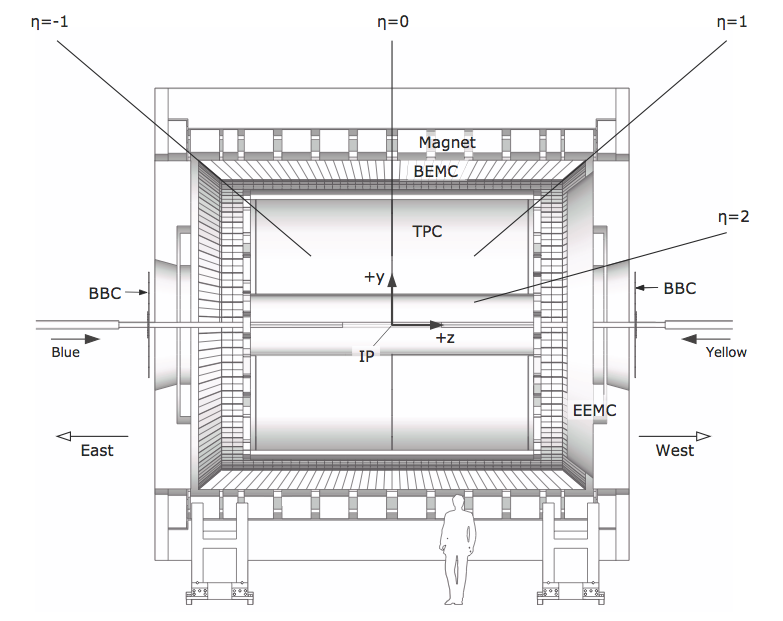
\includegraphics[width=1.0\textwidth]{figures/star-schematic-new}
  \caption{Schematic overview of the STAR detector, identifying many of the
  detector subsystems and defining the STAR coordinate system.}
  \label{fig:star-schematic}
\end{figure}

\subsection{Trigger System}

STAR has a 3 level hardware trigger system (L0, L2, L3) \cite{Bieser:2002ah,
Adler:2002ab} allowing for the selection of rare events from the large pool of
minimum bias (MB) interactions. While the TPC and other tracking detectors
have long readout times compared to the interaction rate, the BBCs and the
BEMC are fast detectors that sample each bunch crossing at the STAR IR, and
can thus be used for efficient selection of high $p_T$ events. A typical
trigger mix consists of $\sim$10-20 separate triggers running in parallel.
Significant improvements to the STAR data acquisition system (DAQ) beyond
design specifications have increased the rate of event recording to typical
values of 30-50 Hz, with a dead-time fraction of $\sim$50\%.

The L0 trigger operates on coarse-granularity data from fast detectors and
builds a decision tree capable of completing its analysis in time with the 119
nanosecond RHIC bunch crossing interval. If the L0 trigger issues an accept
the full trigger detector data is sent to L2 for further analysis. In contrast
to L0, the L2 trigger runs on commodity hardware and its algorithms can be
written in C. It applies preliminary calibrations and can do some primitive
jet finding in the course of making its decision, but must issue that decision
in no more than 5 milliseconds. If the L2 trigger issues an accept, the slow
detectors are read out and the full event is recorded to tape. The L3 trigger
\cite{Adler:2002ab} enables online TPC track finding using a farm of commodity
servers. It was at one time a necessary component of the trigger system, but
upgrades to the data acquisition system have increased the throughput from
STAR to the RHIC Computing Facility (RCF) to the point where the $\sim$50 Hz
of events selected by the L0 and L2 trigger algorithms can be recorded to
tape. The L3 tracking output continues to serve as a useful qualitative
monitoring tool in the STAR control room.

\subsection{Beam Beam Counters\label{sec:bbc}}

The BBCs \cite{Kiryluk:2003aw} consist of two hexagonal scintillator arrays,
one immediately outside each magnet poletip 3.7~m from the interaction point.
Each array is tiled from 36 individual hexagonal scintillators read out by
wave length shifting fiber and a photomultiplier tube. The beam pipe passes
through the center of the array. The region 9.6~cm to 48~cm from the beam axis
($3.3 < |\eta| < 5.0$) is covered by 18 small hexagonal tiles. The remaining
region out to 193~cm from the beam pipe ($2.1 < |\eta| < 3.3$) is covered by
18 large hexagonal tiles. Only the small tiles are used in this analysis.
Thresholds are set well below the signal deposited by a single ionizing
particle in a tile, and a bunch crossing is recorded as having a hit based on
the relative timing between the first signal from any of the small tiles on
one side with the first signal from any of the small tiles on the other. The
timing resolution is $\sim$1~ns, sufficient to separate beam backgrounds which
should hit the two counters in succession vs. particles from a collision which
should result in both counters being struck simultaneously. A timing cut 8~ns
wide selects only coincidences with collision timing, and individual scalers
are kept for each timing bin in addition to the total in the timing gate, thus
allowing for more selective cuts offline.

In addition to defining the MB trigger condition, coincident signals in the
BBCs also serve as a luminosity monitor. In particular, tracking the number of
BBCs hits per bunch crossing allows one to measure the luminosities for each
combination of the spin states of the two beams. The ratios of these
luminosities are a crucial element in the extraction of single- and
double-spin physics asymmetries at RHIC. The absolute luminosity seen by the
BBCs is calibrated by measuring the size of the beams and the number of
colliding protons. The coincident cross section was found to be 26.1 $\pm$
1.8(stat) $\pm$ 1.8(syst)~mb, representing $87\pm8\%$ of the non-singly
diffractive pp cross section \cite{Adams:2003kv}. This translates into a
typical BBC coincidence rate for 2005(2006) data of $\sim$180(??)~kHz.

\subsection{Zero Degree Calorimeters\label{sec:zdc}}

The ZDCs \cite{Adler:2003sp} are hadron calorimeters placed 18~m upstream on
each side of the the STAR interaction point. This places them on a line with
the colliding beams but outside the final bending magnets between the two beam
lines. They are 6 hadronic interaction lengths in depth but only 10~cm wide
extending $\pm$2.7~mrad from the beam. As with the BBCs, a hit is recorded
based on a coincidence between the two ZDCs with timing consistent with
particles arriving simultaneously from the interaction point. These devices
are designed to be sensitive to neutrons from heavy ion reactions and thus are
not used as trigger detectors in the pp program. They do serve as a secondary
luminosity monitor useful for many systematic error checks. They typically
count a factor of 100 less than the BBC.

\subsection{Scaler System\label{sec:scalers}}

Signals from the L0 Trigger and the BBCs and ZDCs are processed by a set of 12
Scaler Boards \cite{scalers}. A Board is a custom VME histogramming module with
24 input bits, the combination of which maps to one of \(2^{24}\) 40 bit memory
locations on the module. 7 input bits are reserved for an encoding of the bunch
crossing number, leaving 17 for detector-specific logic. The memory location
addressed by a particular 24 bit input pattern is incremented when an event
satisfies that bit pattern. The scaler system typically tracks hits in the East
and West halves of the luminosity monitors separately, as well as a variety of
coincidences with different \(\Delta T\) requirements. Some of the boards are in
continuous operation during a STAR run, while others sample at discrete
intervals.

\subsection{Electromagnetic Calorimeters}

Electromagnetic calorimetry is an essential element of the trigger system at
STAR and is also important for many final state analyses (especially, for the
purposes of this thesis, jet reconstruction). We will focus on two calorimeter
subsystems: the BEMC \cite{Beddo:2002zx}, covering $|\eta| < 1.0$, and the
EEMC \cite{Allgower:2002zy}, which is installed only on the West side of STAR
and spans $1.09 < \eta < 2.0$. Both the BEMC and EEMC are segmented sampling
calorimeters with lead absorber layers and active plastic scintillator layers.
The BEMC is divided into 4800 projective towers spanning $\Delta \eta \times
\Delta \phi = 0.05 \times 0.05$, while the EEMC's 720 projective towers each
span 0.1 in azimuth and range in pseudorapidity coverage from $\Delta \eta =
0.057$ at $\eta = 1.09$ to $\Delta \eta = 0.099$ at $\eta = 2.0$. Both
calorimeters have a depth of at least twenty radiation lengths.

At Level 0, the BEMC and EEMC implement trigger conditions based on thresholds
in single high towers, 4x4 (4x2) trigger patches, and 20x20 (12x10) jet
patches. At Level 2 the calorimeters drive a wide variety of trigger
algorithms ranging from dijet reconstructions that span seamlessly across the
two calorimeters to heavy flavor searches doing online calculations of tower
pair invariant masses. The primary calorimeter trigger condition used in this
work is the BEMC jet patch (JP) trigger, which requires an energy sum above
threshold in one of twelve fixed collections of 400 towers each spanning
$\Delta \eta \times \Delta \phi = 1.0 \times 1.0$. In this case the Level 2
trigger algorithm is a simple accept, and the EEMC is used only for final
state jet reconstruction.

%% This table is probably not a good idea anyway.
% \begin{table}
%   \begin{center}
%     \begin{tabular}{c|cc}
%       & BEMC & EEMC\\
%       \hline
%       depth & $\geq 20~\chi_0$ & $\geq 20~\chi_0$
%     \end{tabular}
%   \end{center}
%   \caption{PID Selection Windows}
%   \label{tbl:pid-selection-windows}
% \end{table}

\subsection{Time Projection Chamber}

The TPC \cite{Anderson:2003ur} is the primary detector subsystem at STAR,
providing full azimuthal tracking of charged particles with transverse
momentum above $\sim 100$ MeV/c and $|\eta| < 1.8$, and particle
identification through measurements of ionization energy loss. It is a 4.2
meter long volume of gas bounded by an inner field cage at a radius of 50
centimeters and an outer field cage at 200 centimeters. The end caps of the
detector are held at ground potential and the central cathode membrane at
-28kV; metal rings connected by precision resistors in the field cages ensure
a uniform electric field of $\approx 135$ V/cm. The TPC sits inside a solenoid
with a field strength of 0.5 Tesla.

Charged particles ionize the P10 gas as they traverse the volume of the TPC,
producing secondary electrons that drift to the nearest end cap of the
detector. The $z$ coordinate of each point along the track is calculated by
measuring the time required for the electrons to reach the end cap and
dividing by the drift velocity. The drift velocity varies with electric field
strength and with the temperature, pressure, and composition of the gas, so
measurements of it are performed every few hours using the TPC laser system
\cite{Abele:2003aa}. Radial laser beams at known positions along the length of
the TPC ionize trace organic substances in the P10 gas; the time difference
between the arrival of electrons liberated by lasers at two different
positions allows a calculation of the drift velocity.

% could say a little more about how electron drift time is measured ... e.g. time buckets for readout pads
Each end cap is divided into twelve sectors, positioned as the hours on a
clock face, and each sector contains 45 rows of cathode pads (5,692 pads per
sector). The cathode pads are mounted on anode wires; the secondary electrons
avalanche near the anode wires, and the positive ions produced in this
avalanche generate a temporary image charge on several nearby pads. The image
charge is measured, and an analysis of the charge sharing between the pads
allows the original track $x$ and $y$ coordinates along the wire to be
reconstructed to within a small fraction of a pad width. Finally, the charge
deposited on each pad is used to calculate the particle's energy loss per unit
length due to ionization, or dE/dx.

\begin{figure}
  \includegraphics[width=1.0\textwidth]{figures/tpc}
  \caption{The STAR Time Projection Chamber (TPC). The end-caps are divided
  into twelve sectors, each with an inner and outer sub-sector. The TPC is
  divided into two by a central cathode membrane spanning the gas volume
  between the inner and outer field cages.}
  \label{fig:tpc}
\end{figure}

\subsection{Computing Facilities}

The aggregate raw data produced by all detector subsystems in STAR is on the
order of 100 MB per event. The STAR Data Acquisition System (DAQ)
\cite{Landgraf:2002zw} reduces the event size through hardware-based zero
suppression, resulting in a 10x savings for the highest multiplicity heavy ion
collisions and substantially greater savings (100x or more) for the
proton-proton collisions analyzed in this work. It then organizes the data
into DAQ files and transfers these files to tape in the RHIC Computing
Facility's HPSS hierarchical storage system, which provides 8 PB of storage
and a throughput of over 300 MB per second to the RHIC and USATLAS
experiments.

Event reconstruction and data analysis takes place on a Linux compute farm
with over 3300 cores and 1.7 PB of local storage. The STAR reconstruction
software is written in C++ and runs on Scientific Linux, a version of Red Hat
Enterprise Linux maintained by the particle physics community. The event
reconstruction code loads DAQ files from HPSS into local storage, performs
tracking and applies a variety of detector calibrations, and generates ``micro
Data Storage Tapes'' or ``$\mu$DSTs'', which contain higher-level physics
objects such as particle tracks, event vertices, and calorimeter clusters.
$\mu$DSTs are implemented using ROOT \cite{Brun:1997pa} TTrees, allowing
efficient ad-hoc and batch data analysis. The analysis presented here was
performed on a set of TTrees generated from $\mu$DSTs using a mix of custom
C++ libraries and Python scripts interfacing with the ROOT data analysis
framework.

\chapter{Event Reconstruction}
\input{ch3-00-monte-carlo}
\section{Triggering and Data Acquisition}

The basic building block of nearly all physics analyses in the 200 GeV pp
program is the minimum-bias (MB) trigger defined by coincident signals in the
East and West BBCs, yielding a sensitivity of 26.1$\pm$2.0 mb (87\%) of the
NSD cross section as deduced from a Vernier scan performed in 2003. On top of
the MB trigger STAR layers a variety of requirements based on signals in the
electromagnetic calorimeters that bias the event sample towards rare events
with large transverse energy depositions.

The dominant trigger algorithm in this analysis is the BEMC jet patch (JP)
trigger, which sums transverse energy depositions over fixed groups of 400
towers covering an area of $\Delta \eta \times \Delta \phi$ = 1.0 $\times$
1.0. The JP trigger is designed for efficient, minimally-biased selection of
high-energy jets. The threshold for the primary JP trigger in the 2005 (2006)
run was 6.4 (8.3) GeV, and the trigger sampled an integrated luminosity during
longitudinal running of 3.3 (6.8) $pb^{-1}$.

% The 8.3 number excludes transverse running.  Including that the 06 number would be 1.95 (1st long) + 3.20 (trans) + 6.30 (2nd long) = 11.45
% also assumes a MB cross section of 25 mb, not 26.1 as stated here
% http://www.star.bnl.gov/protected/common/common2006/trigger2006/lum_pertriggerid_pp2006.txt

% 2006 DSM prescales
% mysql --host=dbbak.starp.bnl.gov --port=3405 Conditions_rts
% SELECT run.idx_rn, dict.value FROM dict,run WHERE dict.hash=run.dicthash AND dict.label='mb-prescale' AND run.idx_rn<7160000 AND dict.value>0;

% Regular prescales, event counts (port 3404 for 05, port 3405 for 06)
% mysql --host=dbbak.starp.bnl.gov --port=3405 RunLog
% SELECT run, offlineTriggerID, prescale, numberOfEvents FROM l0TriggerSet;

% my thresholds assume final calibrations, I think

% Jamie's integrated lumi numbers are somewhat smaller than mine, presumably because of some basic quality cuts.  My numbers for 06 BJP1 are

% 117221 2.4
% 127221 3.6
% 137221 0.1
% 137222 6.8

% for a total sampled lumi from longitudinal running of 9.3, rather than 8.3

\input{ch3-02-tracking}
\section{Vertexing}

STAR uses different vertex finders optimized for the very different running
conditions of heavy ion (MinuitVF) and proton-proton (PPV) collisions. A
detailed description of both can be found in STAR Note 488
\cite{vertex-finder-starnote}; the discussion here will focus on the Pile-Up
Proof Vertexer (PPV), but many of the basic principles apply to both
algorithms.

One of PPV's major design goals is robustness in the face of high levels of
pileup. Pileup events usually occur in one of the $\sim$40 other bunch
crossings that are read out along with the trigger bunch crossing by the TPC,
although on rare occasions a single bunch crossing can contain multiple hard
scatterings. PPV does not try to guard against this in-time pileup, but it
does work to suppress false event vertices from other bunch crossings.

PPV relies on a pre-calculated beam line constraint for the $x$ and $y$
position of each vertex. The beam line constraint is determined by running the
Minuit Vertex Finder on a subset of high-multiplicity events and fitting the
resulting distribution of event vertices with a straight line. PPV uses a
subset of TPC tracks satisfying a series of quality cuts; these include a
transverse momentum greater than 200 MeV, a distance of closest approach (DCA)
to the beam line of less than 3 cm, and a requirement that the number of hits
used to fit the track is at least 70\% of the maximum number of possible hits
for the track's helix. Each track is given an initial weight based on
projection of its DCA in the $xy$ plane and the errors on the extrapolation to
the beam line used to calculate that DCA. The track's weight is increased if
it is reconstructed from a minimum number of hits on both sides of the central
membrane of the TPC or is matched to an energy deposit in the BEMC or EEMC,
since tracks satisfying one or more of those conditions are very likely to
have been produced in the bunch crossing that fired the trigger(s). A track
with one of these positive weight adjustments is called a ``matched'' track.
Conversely, if a track extrapolates to an active calorimeter tower without any
energy deposit, or crosses the central membrane but has fewer than the minimum
required number of hits on both sides of the membrane, the track's weight is
reduced. The total weight for the track is the product of the initial weight
and each of these adjustments.

Vertices are identified by binning the $z$ axis with 1mm resolution and
generating a histogram of all the track weights. The peak of the histogram is
the first vertex candidate; all tracks which extrapolate to within 3cm of this
vertex position are grouped with the candidate and removed from further
analysis. PPV iterates this procedure until no more vertex candidates can be
found. In the 2005 and 2006 runs PPV required at least two ``matched'' tracks
in order to save a vertex; that requirement has been relaxed in recent years
to improve the vertex finding efficiency for forward triggers, which have
event topologies that make it unlikely to find two tracks in an event
satisfying the matching conditions. PPV saves multiple vertices for each
event, ordered by rank; in 2005 and 2006, the rank is simply the cumulative
weight of all the tracks in the vertex. The vertex finding efficiency is
highly trigger-dependent; Table \ref{tbl:vertex-finding-efficiencies} lists
the fraction of events with at least one primary vertex in each of the
triggers used for this analysis.

\begin{table}
  \begin{center}
    \begin{tabular}{cc|rrr}
      \hline
      year & trigger ID & total events & events with vertex & efficiency\\
      \hline
      \hline
      2005 & MB (96011) & 1,686,762 & 1,084,203 & 64.3\%\\
      \hline
      2005 & BJP1 (96221) & 1,878,465 & 1,835,016 & 97.7\%\\
      \hline
      2005 & BJP2 (96233) & 5,446,354 & 5,243,167 & 96.3\%\\
      \hline
      2006 & MB (117001) & 257,291 & 131,657 & 51.2\%\\
      \hline
      2006 & BJP1 (13722[1-2]) & 3,294,257 & 3,138,997 & 95.3\%\\
      \hline
    \end{tabular}
  \end{center}
  \caption{Vertex Finding Efficiencies for events analyzed in this work.}
  \label{tbl:vertex-finding-efficiencies}
\end{table}

Once the vertices have been identified, the tracker adds the vertex position
as an additional hit to every track associated with that vertex and refits
those tracks. The STAR software framework saves this collection of ``primary''
tracks as well as the original ``global'' tracks. In this analysis primary
tracks are used exclusively; the global tracks associated with those primaries
are only analyzed to apply a more stringent cut on the DCA to the primary
vertex position obtained from the original track extrapolation.

\begin{figure}
  \includegraphics[width=1.0\textwidth]{figures/ppv-candidate-distribution}
  \caption{Example vertex candidate distribution generated by PPV
  \cite{vertex-finder-starnote}. An ordered list of vertices is extracted from
  the peaks of this distribution, with the requirement that each vertex
  contains at least two tracks satisfying the matching conditions.}
  \label{fig:ppv-candidate-distribution}
\end{figure}

\section{Spin Sorting\label{sec:spindb}}

Each of the bunches in the two RHIC beams is polarized independently, and the
polarization pattern can change from fill to fill. An accurate record of the
spin state of each bunch crossing in a fill is essential for any spin
analysis. The polarization pattern for the rings is set by the RHIC
Collider-Accelerator Department (C-AD) and broadcast through the CDEV
\cite{Barton:2003sh} control and monitoring system. The pattern is formatted
as a list of 360 8 bit numbers, one for each of the time buckets in RHIC, and
is defined in terms of the bunch crossings at the 12 o'clock position in the
RHIC ring. The beam experiences an odd number of spin flips in between 12
o'clock and the STAR IP at six o'clock, so the beam polarizations at STAR are
flipped relative to the broadcast record. The interpretation of each bit is
given in Table \ref{tbl:spin8}.

\begin{table}
  \begin{center}
  % \begin{ruledtabular}
    \begin{tabular}{c|l}
      \hline
      bit & meaning \\
      \hline
      \hline
      0 & yellow beam filled\\
      \hline
      1 & yellow beam polarized up\\
      \hline
      2 & yellow beam polarized down\\
      \hline
      3 & yellow beam unpolarized\\
      \hline
      4 & blue beam filled\\
      \hline
      5 & blue beam polarized up\\
      \hline
      6 & blue beam polarized down\\
      \hline
      7 & blue beam unpolarized\\
      \hline
    \end{tabular}
  % \end{ruledtabular}
  \end{center}
  \caption{Significance of each of the bits in an eight bit spin record.}
  \label{tbl:spin8}
\end{table}

A given bunch from the Blue ring always collides with the same bunch from the
Yellow ring at a specific interaction point in the RHIC ring over the course
of a fill. C-AD has historically configured the beams so that bunch zero from
the Blue beam collides with bunch zero from the Yellow beam at the PHENIX IP,
and as a result the PHENIX experiment sees only one abort gap in its fill
patterns. The situation is different at STAR, where the RHIC ``toggle mode''
defines the pairs of bunches from the Blue and Yellow beams that collide. The
toggle mode is typically set once at the beginning of the RHIC data-taking
period, and is encoded implicitly in the spin patterns broadcast by CDEV.

After accounting for the spin flip and the toggle mode, an analysis must map
the event IDs recorded at the experiment to the 7 bit bunch crossing IDs
defined by CDEV in order to determine the spin state of a given event. The
STAR Trigger receives this information from RHIC for every event, but analyses
have observed occasional inaccuracies in the feed that render it unreliable.
Instead, STAR uses a more robust 48 bit counter synchronized to the 9.4 MHz
RHIC clock to uniquely identify every event. The 7 bit bunch crossing IDs can
be expressed in terms of this 48 bit counter as
%
\begin{equation}
  \mathrm{7~bit~ID} = \left(\mathrm{48~bit~counter} + \mathrm{offset}\right)~mod~120
\end{equation}
%
The offset is calculated for each STAR run by generating 120 histograms of
triggers versus the 7 bit bunch IDs for each possible value of the offset,
comparing these histograms to a histogram of the intended spin pattern at
STAR, and searching for a minimum in the $\chi^2$ distribution. An example of
the overlap between the trigger rate versus bunch crossing ID and the spin
pattern after the correct offset has been applied is shown in Figure
\ref{fig:bxing-offset}. The offsets for each STAR run are calculated once and
uploaded to the STAR Calibrations DB which allows them to be applied by all
STAR spin analyses. Further details of the spin state determination can be
found in Reference \cite{spin-db-website}.

\begin{figure}
  \includegraphics[width=1.0\textwidth]{figures/bxing-offset-determined}
  \caption{Distribution of events (blue) versus the corrected 7 bit bunch
  crossing IDs at the STAR interaction point. The yellow bars indicate the
  bunch crossings where both beams have filled bunches according to the
  intended spin patterns broadcast by CDEV.}
  \label{fig:bxing-offset}
\end{figure}

\section{Jet Finding}

\subsection{Clustering Algorithm}

STAR has implemented the midpoint-cone algorithm in accordance with the
recommendations of Reference \cite{Blazey:2000qt}. The algorithm proceeds by
assembling a $p_{T}$ ordered list of four momenta (``protojets") for each
event. Each protojet with $p_T>p_{T}^{seed}$ (``seeds") initiates a clustering
sequence. For each clustering sequence, protojets within an angular distance
$\Delta r = \sqrt{\Delta\phi^{2} + \Delta\eta ^{2}} < r_{cone}$ are selected
and their four momenta are added to define the four momentum of the cluster
via $p_{\mu}^{cluster} = \sum p_{\mu}^{i}$. If $p_{\mu}^{cluster}$ lies within
a distance $\epsilon$ of the initiating protojet, the clustering sequence
terminates. Otherwise the clustering sequence is iterated about the direction
$p_{\mu}^{cluster}$ until convergence is reached. Once stable configurations
are identified, the association is cataloged for later use. However, no
protojets are removed from the sample. Clustering continues until the list of
seeds is exhausted, yielding a list of redundant, overlapping, stable
clusters. Before disentangling the stable clusters, the algorithm first tests
for missed initiating directions by constructing a set of test seed directions
at the ``midpoint" between all possible pairs of neighboring clusters.
Specifically, locations at the midpoint of all cluster pairs separated by
distance $d < 2 \times r_{cone}$ are tested for stable cluster configurations.
Clusters formed around midpoint seeds are only retained if the resulting
cluster lies within $\epsilon$ of the midpoint seed, and no iteration is
performed.

After all midpoint seeds have been tested, the resulting list of stable
clusters is disentangled via a splitting/merging algorithm. The algorithm
proceeds by finding the highest $p_{T}$ cluster, referred to as the ``root"
cluster. Next, all clusters sharing protojets with the root cluster
("neighbors") are identified, and the neighbor with the largest $p_T$ is
selected. The root and neighbor jet are merged if
$\frac{p_{T}^{shared}}{p_{T}^{neighbor}}>f_{split-merge}$ where $0 <
f_{split-merge} < 1$. If this condition is not satisfied the clusters are
split such that each protojet is assigned to the closest of the two
overlapping clusters. After each split/merge, the cluster list is again sorted
by $p_T$, a new root cluster is chosen, and the splitting/merging continues
until no protojets are shared amongst clusters. It is important to note that
the split/merge step takes a list of clusters that are essentially circular,
while the final clusters are no longer necessarily circular. Finally, each of
the unique clusters is tagged as a ``jet", whose four momentum is the vector
sum of the constituent protojets.

\subsection{Application at STAR}

STAR applies the midpoint-cone algorithm to cluster charged particle tracks
and BEMC tower energies as follows. Charged particle protojets are constructed
from all primary TPC tracks satisfying the aforementioned cuts. A charged pion
mass is assumed when relating energy and momentum. Each BEMC tower energy
measurement is corrected for charged particle energy deposition by i)
identifying the number of TPC tracks projecting to the tower and ii)
subtracting the most probable MIP energy deposition for each of the projecting
tracks. After MIP subtraction, each tower energy measurement is converted to a
four momentum using knowledge of the highest-ranking primary vertex location
and assuming a photon mass. Protojets are then constructed for towers with
corrected $E_{T}>0.2 $GeV.

The midpoint-cone algorithm first sorts the protojets onto a grid of
$\Delta\eta=\Delta\phi=0.05$, where the properties of each grid ``cell" are
defined by the vector sum of its constituent protojets. This discretization
improves computational efficiency and minimizes potential biases arising from
the fact that the BEMC towers may measure energy from more than one particle.
Each cell maintains a list of its constituent protojets so that there is no
ultimate loss of information. The midpoint cone algorithm then operates on the
list of cells, and after clustering and splitting/merging conclude, each
cluster is then characterized by the vector sum of its constituent four
momenta. Jets with $p_{T}<5$ GeV/$c$ are discarded. The control parameters of
the clustering algorithm are listed in Table \ref{tbl:jetfinding-parameters}.
The restricted cone radius in the 2005 analysis was motivated by the limited
pseudorapidity acceptance of the partially installed BEMC.

\begin{table}
  \begin{center}
    % \begin{ruledtabular}
      \begin{tabular}{|c|c|c|}
        \hline
        Parameter & Value \\
        \hline
        cone radius  &   0.4 (2005), 0.7 (2006) \\
        seed $p_{T}$ threshold  &   0.5 GeV/$c$ \\
        $f_{split-merge}$  &  0.5  \\
        clustering convergence distance $\epsilon$  &  0.025  \\
        \hline
      \end{tabular}
    % \end{ruledtabular}    
  \end{center}
  \caption{Control parameters used in midpoint-cone clustering and described in detail in the text.}
  \label{tbl:jetfinding-parameters}
\end{table}

\section{Charged Pion Identification \label{sec:pid}}

Charged pions are identified and separated from kaons, protons, and electrons
by the amount of energy they lose in the TPC. The dE/dx of a TPC track is
obtained by sorting the track hits according to energy loss, removing the top
30\%, and averaging the rest. Track dE/dx values for a given particle species
at a fixed momentum are Gaussian, so one can also express the dE/dx value for
each track in terms of a deviation from the mean dE/dx for some identified
particle at that track's momentum. In particular, track energy loss values at
STAR are commonly given in terms of ``$n\sigma(\pi)$'', the deviation from the
mean of the pion peak divided by the width of said peak. Protons and kaons
fall to the left of the pion peak (lower energy loss) and electrons fall to
the right (higher energy loss).

The peak position of the raw $n\sigma(\pi)$ distribution generated by the STAR
reconstruction software exhibits some significant time dependence, so instead
of assuming a fixed mean of 0.0 for the pion Gaussian, this analysis performs
a triple Gaussian fit on the $n\sigma(\pi)$ distribution for each fill and
extracts time-dependent means to better calibrate the PID cut. After this
recalibration one can extract yields for the various species of charged
particles by fitting the $n\sigma(\pi)$ distributions with a multi-Gaussian
parametric function. The fitting procedure starts with 8 Gaussians -- one each
for $\pi^{+}$, $\pi^{-}$, $K^{+}$, $K^{-}$, $p$, $\bar{p}$, $e^{+}$, and
$e^{-}$. The number of free parameters is reduced by applying the following
constraints:

\begin{itemize}
    \item all widths must be equal (dE/dx resolution isn't particle-dependent)
    \item particle/antiparticle pairs should have the same mean
    \item $\pi - K$, $\pi - p$, and $\pi - e$ separations are known from other analyses \cite{Xu:2008th}
\end{itemize}

In the end there are 24 - 7 - 4 - 3 = 10 free parameters in the fit: the
Gaussian width, the position of the $\pi$ Gaussian, and the yields. The
particle separations change as a function of momentum, not $p_{T}$, so we
slice a $p_{T}$ bin into momentum bins and fit each one individually. Figure
\ref{fig:typical-nsigmapi} shows a typical fit result. The tracks have been
shifted by 6*charge in order to plot positive and negatively charged tracks on
the same histogram.

\begin{figure}
  \begin{center}
    \includegraphics[width=0.7\textwidth]{figures/typical-nsigmapi}    
  \end{center}
  \caption{Example PID fit result}
  \label{fig:typical-nsigmapi}
\end{figure}

With this database of particle yields in hand we can calculate the set of PID
cuts that minimize the statistical uncertainty on the background-subtracted
$A_{LL}$ (Equation \ref{eqn:sigma-all}). A simple minimization routine
assuming $\sigma_{A_{LL}}^{2} = 1/N$ for the raw asymmetries yields the
results in Table \ref{tbl:pid-selection-windows}.

\begin{table}
    \begin{center}
        \begin{tabular}{c|ccc}
        \hline
        $p_{T}$ bin & $\pi$ window & proton/kaon max & electron min\\
        \hline
        \hline
        [2.00 - 3.18] & (-1.10, 2.30) & -2.10 & 2.60\\
        \hline
        [3.18 - 4.56] & (-1.40, 2.10) & -2.10 & 2.40\\
        \hline
        [4.56 - 6.32] & (-1.40, 1.80) & -2.10 & 2.40\\
        \hline
        [6.32 - 8.80] & (-1.40, 1.80) & -2.10 & 2.40\\
        \hline
        [8.80 - 12.84] & (-1.30, 1.40) & -2.10 & 2.10\\
    \hline
    \end{tabular}
    \end{center}
    \caption{PID Selection Windows}
    \label{tbl:pid-selection-windows}
\end{table}


\chapter{Analysis}

The analysis encompasses data taken during the 2005 and 2006 RHIC runs when
the polarized proton beams were longitudinally polarized and colliding at a
center-of-mass energy of 200 GeV. Spin asymmetries are constructed using
charged pions produced at mid-rapidity and having large transverse momentum.

\section{$A_{LL}$ Methodology}

We begin with the equation for a double spin asymmetry in terms of directly measurable quantities,
%
\begin{equation}
  A_{LL} = \frac{\sum_{runs} P_{Y}P_{B}\left[(N_{uu} + N_{dd}) - R(N_{ud} + N_{du})\right]}{\sum_{runs} P_{Y}^{2}P_{B}^{2}\left[(N_{uu} + N_{dd}) + R(N_{ud} + N_{du})\right]}.
  \label{eqn:all-basics}
\end{equation}
%
Henceforth parity conservation is employed; the \(++\) subscript denotes a sum
over the \(uu\) and \(dd\) states and the \(+-\) subscript a sum over \(ud\)
and \(du\) states. \(P_Y\) and \(P_B\) are the Yellow and Blue RHIC beam
polarizations, \(N_{ij}\) are spin-dependent charged pion yields, and \(R =
\frac{\mathcal{L}_{++}}{\mathcal{L}_{+-}}\) is a ratio of sampled luminosities
in different spin configurations. Each of the $\mathcal{L}_{ij}$ is a sum of
the scaler counts over bunch crossings with that spin state.

The formula for the statistical uncertainty on \(A_{LL}\) neglects
uncertainties on the relative luminosities and beam polarizations. Assuming
Poisson statistics on \(N_{++}\) and \(N_{+-}\) the uncertainty on the
asymmetry for a single run is
%
\begin{equation}
  \left(\frac{\sigma_{A_{LL}}}{A_{LL}}\right)^2 = \left(N_{++} + R^2 N_{+-}\right)\left[\frac{1}{N^2} + \frac{1}{D^2} - \frac{2 \times COV(N,D)}{ND} \right]
\end{equation}
%
where \(N\) and \(D\) are the numerator and denominator of the raw asymmetry
(that is, neglecting polarizations), and \(COV(N,D) = N_{++} - R^2 N_{+-}\).
In the case of small asymmetries \(\frac{1}{N^2} \gg (\frac{1}{D^2} - \frac{2
COV(N,D)}{ND}\)), and the uncertainty on the numerator dominates the uncertainty
on \(A_{LL}\):
%
\begin{equation}
  \left(\frac{\sigma_{A_{LL}}}{A_{LL}}\right)^2 \approx \frac{N_{++} + R^2 N_{+-}}{N^2}
\end{equation}
%
ROOT's TH1::Divide method does the error propagation correctly in this limit
(it ignores the covariance term). The generalization to a sum over runs is
straightforward since the yields for each run are uncorrelated.

\subsection{Multi-Particle Statistics}

This analysis often accepts multiple pions from a single event. Treating each
of the particles as an independent event and na\"ively using
$\sqrt{N_{pions}}$ for the statistical uncertainty as in the previous section
is not correct. Following the prescription in
\cite{sowinski-multiparticle-statistics} each bin in a histogram is
incremented at most once per event, using a weight equal to the number of
particles that fell into the bin. This technique neglects intra-event particle
correlations across histogram bins.

\subsection{Background Subtraction}

As discussed in Section \ref{sec:pid}, a particle's energy loss per unit path
length (dE/dx) in the TPC provides an effective means of identification across
a broad range of momenta. In the momentum range of interest (2.0 GeV/c and up)
charged pions are not fully separated from heavier charged hadrons (primarily protons and kaons, which have a smaller \(\langle dE/dx \rangle\)) and
electrons (which have a larger \(\langle dE/dx \rangle\)). This contamination is addressed by subtracting the asymmetry of
the background from the raw asymmetry calculated using all
particles in the charged pion acceptance window. The background sidebands located on both sides of the acceptance window have different physical sources and potentially different double spin asymmetries.  The subtraction
procedure must also account for the lack of a clean background sample; the
sidebands themselves have a non-negligible contamination from the charged pion
signal. We start by defining a reduced background fraction to account for the
impurities in the sideband:

\begin{equation*}
  f_{x}(y) = \frac{x~\mathrm{counts~in}~y~\mathrm{window}}{\mathrm{total~ in}~y~\mathrm{window}}
\end{equation*}

\begin{equation*}
  f'(x) = \frac{f_{x}(\pi)}{1 - f_{\pi}(x)}
\end{equation*}
%
The standard equations for the background-subtracted $A_{LL}^{\pi}$ and its
statistical uncertainty are only modified by replacing the background fraction
for each sideband with its reduced background fraction:

\begin{equation}
  A_{LL}^{\pi} = \frac{ A_{LL}^{\pi,raw} - f'(p+K)A_{LL}^{p+K,raw} - f'(e)A_{LL}^{e,raw} }{1 - f'(p+K) - f'(e) },
  \label{eqn:all}
\end{equation}

\begin{equation}
  \sigma_{A_{LL}^{\pi}} = \frac{\sqrt{ \sigma_{A_{LL}^{raw}}^{2} + f'(p+K)^{2} * \sigma_{A_{LL}^{p+K,raw}}^{2} + f'(e)^{2} * \sigma_{A_{LL}^{e,raw}}^{2} }}{1 - f'(p+K) - f'(e)}.
  \label{eqn:sigma-all}
\end{equation}
%
These equations are the final formulae used to calculate the asymmetries for a single STAR run in this work.  The \(raw\) superscript in the formulae denotes an \(A_{LL}\) calculated without background subtraction but taking multi-particle statistics into account.

Equation \ref{eqn:all-basics} specified beam polarizations, spin-dependent relative luminosities, and spin-sorted particle yields as the three components to a double spin asymmetry measurement.  A discussion of the extraction of each of these quantities follows.
\section{Beam Polarizations}

Time-dependent relative beam polarizations are obtained from the pC CNI
polarimeter and normalized by the H-jet polarimeter. pC measurements are made
every few hours during a fill, while the H-jet polarimeter is taking data
almost continuously.

During the 2005 RHIC run pC measurements were generally performed with
vertical targets at one location in \(x\), the horizontal coordinate in the
plane transverse to the beams. The intent was that the measurement be made at
the intensity peak. A small number of explicit polarization profile
measurements were also performed. A study of the normalized event rates
obtained by the polarimeter indicated that the target was occasionally
off-center relative to the beam. In the case of the blue beam, the
polarization showed no dependence on normalized event rate, nor any explicit
dependence on \(x\) in the profile measurements. In contrast, the yellow beam
polarization exhibited a significant normalized rate dependence as well as an
\(x\) dependence in the profile measurements. In the 2006 RHIC run scanning
profile measurements in \(x\) were executed for both beams as the normal mode
of operation as a result of this discovery.

The existence of a non-uniform polarization profile in the beam has
implications for the H-jet normalization procedure. The H-jet target is large
compared to the size of the beam and thus samples the average polarization,
while the pC target is small in one dimension. In order to relate the two one
needs to calculate an average beam polarization from the pC measurements,
which requires knowledge of the beam intensity and polarization profiles in
the transverse dimension orthogonal to the carbon strip. The data from the
2006 polarimeter measurements theoretically enables a direct extraction of
both profiles, but occasional problems with the target positioning render the
procedure somewhat unreliable.

The alternative approach employed by the CNI Polarimeter Group in both the
2005 and 2006 data analyses relies on the assumption that the beam intensity
and polarization profiles are Gaussian with independent widths, and that the
peak of the polarization profile is located at the center of the beam. Then
the polarization \(P\) and normalized event rate \(I\) are related by
%
\begin{equation}
  \frac{P}{P_{max}} = I^R, ~~~~ R=\left(\frac{\sigma_I}{\sigma_P}\right)^2.
  \label{eqn:polarization}
\end{equation}
%
\(P_{max}\) and \(R\) are free parameters determined in a fit to the data (see
Figure \ref{fig:pol_l_lmax}); the average beam polarization in terms of these
parameters is simply
%
\begin{equation}
  \langle P \rangle = \frac{P_{max}}{\sqrt{1+R}}
\end{equation}

\begin{figure}
  \centering
  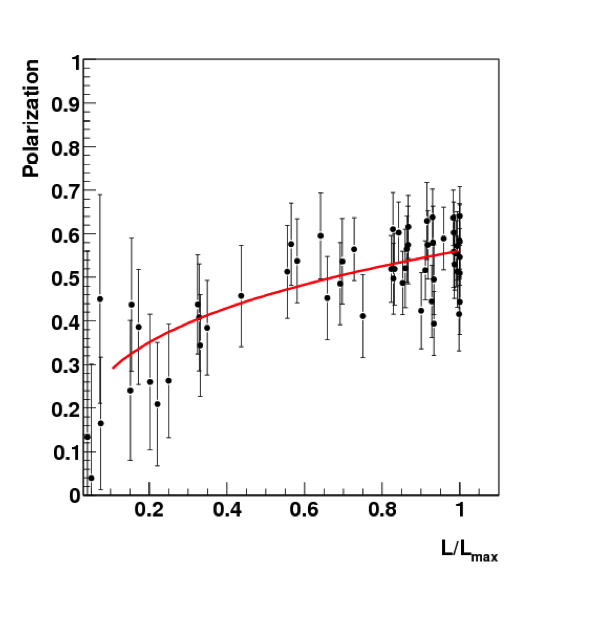
\includegraphics{figures/pol_l_lmax}
  \caption{Example parameterization of beam polarization versus normalized luminosity $I = L/L_{max}$.  The result of the fit is used to calculate the ratio of the widths of the beam intensity and polarization profiles.}
  \label{fig:pol_l_lmax}
\end{figure}

After H-jet normalization, the polarization values reported to the experiments
must be weighted by the product of both beam intensities. Recall that the
value for \(P_{max}\) in \ref{eqn:polarization} already reflects the carbon
ribbon target's uniform cross section in one transverse dimension; the
polarization at the two-dimensional intensity peak is actually
\(P_{max}\sqrt{1+R}\), and the luminosity-weighted average beam polarization
assuming similarly-sized beams (\(\sigma_I^{blue} \approx \sigma_I^{yellow}\))
is then
%
\begin{equation}
  \langle P \rangle_{STAR} = \frac{P_{max} \sqrt{1+R}}{\sqrt{(1+R_x/2)(1+R_y/2)}}.
\end{equation}
%
In the typical pC running mode the carbon ribbon target is vertical, so the
\(R\) in the numerator is more precisely \(R_x\). The polarization profile is
usually much wider than the luminosity profile, so a binomial expansion leads
to
%
\begin{equation}
  \langle P \rangle_{STAR} = P_{max} \sqrt{\frac{1+R_x/2}{1+R_y/2}},
\end{equation}
and in the case where the polarization profiles are similar in both beams, the
luminosity-weighting correction term vanishes. Polarization profile
measurements in the vertical direction are statistically limited in both the
2005 and 2006 datasets but do not indicate any significant difference between
the horizontal and vertical polarization profiles. As a result, the analysis
sets the luminosity-weighting correction term to unity and includes a
systematic uncertainty term reflecting a possible difference in polarization
profiles in the two transverse dimensions.

\begin{figure}
  \subfloat[][Run 5]{
    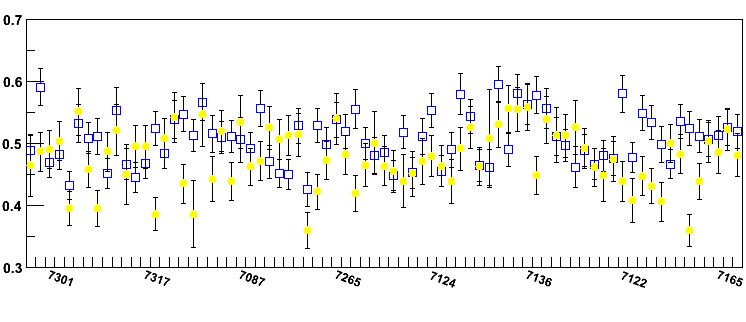
\includegraphics[width=1.0\textwidth]{figures/beam_polarizations_05}
  } \\
  \subfloat[][Run 6]{
    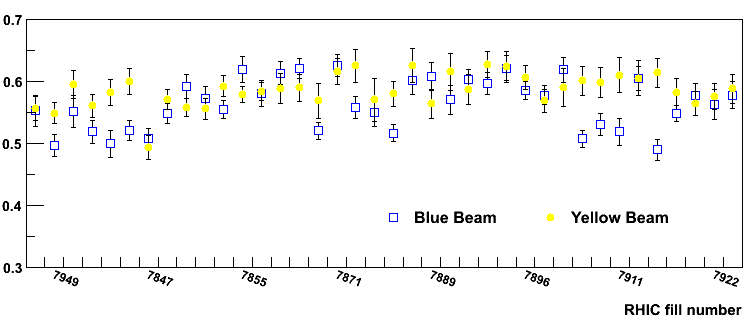
\includegraphics[width=1.0\textwidth]{figures/beam_polarizations_06}
  }
  \caption{RHIC beam polarizations for longitudinally polarized stores analyzed in this work.}
  \label{fig:beam-polarizations}
\end{figure}

The final fill-by-fill beam polarizations are shown in Figure
\ref{fig:beam-polarizations}. The error bars represent statistical and
systematic uncertainties summed in quadrature. The statistical uncertainty for a
fill is obtained by weighting the individual pC measurements in a fill according
to their statistical uncertainty and the duration of time for which the
measurement was ``current''. A variety of sources of systematic uncertainty are
evaluated, including variations in the ``dead layer'' correction that translates
deposited recoil carbon energy to kinetic energy, contributions from molecular
hydrogen in the H-jet target, and imprecise knowledge of the beam polarization
profile. A final tally of the polarizations and their overall uncertainties is
given in Table~\ref{tab:polarizations}. Further details of the analysis can be
found in \cite{CNI05, CNI06}.

\begin{table}
  \centering
  \begin{tabular}{cc|cc}
    \hline
     & & Polarization & Total Uncertainty (dP/P)\\
    \hline
    Run 5 &  Blue & 50.2\% & 5.9\%\\
    Run 5 &  Yellow  & 46.9\% & 6.2\%\\
    Run 5 &  Combined & - & 9.4\%\\
    \hline
    Run 6 &  Blue & 55.9\% & 4.7\%\\
    Run 6 &  Yellow & 58.1\% & 4.8\%\\
    Run 6 &  Combined & - &  8.3\%\\
    \hline
  \end{tabular}
  \caption{Final Beam Polarizations}
  \label{tab:polarizations}
\end{table}

\section{Relative Luminosity Determination}

Bunch-by-bunch beam luminosities are measured using the BBCs and ZDCs and
recorded via the Scaler Boards. The detectors are described in
Sections~\ref{sec:bbc}, \ref{sec:zdc}, and \ref{sec:scalers}. The BBC
measurements are more precise and are employed in the calculation of \(A_{LL}\);
the ZDCs provide a cross-check essential for evaluating systematic
uncertainties.

Various bits of information related to BBC coincidences were encoded on several
Scaler Boards during the 2005 and 2006 RHIC runs. A detailed QA and comparison
of the different boards led to the conclusion that the fine-grained timing
information on boards 5 and 6 should be used to calculate the relative
luminosities. These boards allocated enough bits to track the BBC coincidences
in 16 buckets in \(\Delta T\), the time difference between a hit in the East BBC
and the West BBC. Board 5 was configured to integrate throughout each \(\sim\)
40 minute long STAR run, while board 6 took samples every 250 seconds to allow a
determination of the relative luminosity stability throughout a run.

When possible, the relative luminosities for a run are calculated using the
measurements from board 5. A small number of otherwise-acceptable 2006 runs do
not have reliable scaler information from board 5; in these cases the analysis
relies on the data from board 6. The bunch crossing spin assignments are
obtained using the procedure described in Section \ref{sec:spindb}. The
coincidence count for each bunch crossing is restricted to a set of time buckets
chosen to approximate a 60~cm cut on the $z$ position of the vertex; in the 2005
analysis buckets 7, 8, and 9 are selected, while the 2006 analysis adds bucket 6
into the sum. The relative luminosity \(R\) for a run is then simply the sum of
BBC coincidences in the selected set of time buckets for the bunch crossings
with \(++\) or \(--\) spin assignments divided by the same quantity for bunch
crossings determined to be in a \(+-\) or \(-+\) spin configuration.

% remove runs less than 60 seconds long

% remove runs where the time-integrated BBC coincidence in bit16 < 10k

% remove runs with large number of counts in abort gaps, maybe

% require data from 5/6/11/12, as well as multiple scaler files for the sampling boards

% require that the relative luminosity is fairly stable throughout a fill -- |max(R3) - min(R3)| < 0.0001

% use bit16 on boards 11 and 12, but per-timebin info on boards 5 and 6 (guessing that 11 and 12 don't have timebin info)

% some discrepancies between STAR run stop time and scaler timestamp.  STAR started "getting ahead" of scaler system.  Was anything done about this?  Not clear.  I don't think so

% what was the difference between release 1 and release 2?

\begin{figure}
  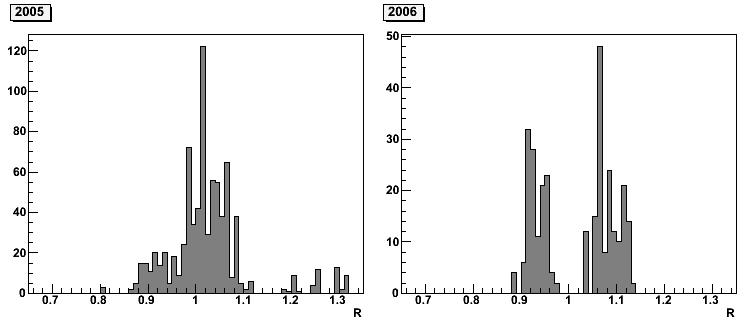
\includegraphics[width=1.0\textwidth]{figures/relative_luminosities}
  \caption{Distributions of per-run values for $R = \frac{\mathcal{L}_{++}}{\mathcal{L}_{+-}}$}
\end{figure}

The statistical uncertainties on $A_{LL}$ assume perfect knowledge of the
relative luminosity of the different spin states. That simplification is
addressed via the systematic uncertainty evaluation described below.

\subsection{Uncertainty Evaluation Using the ZDCs}

% \textit{Note: \href{http://mare.tamu.edu/star/2005n06Jets/2005relLumSys_mar29_2008/}{analysis by Murad Sarsour}}

We can quantify the precision with which we understand the relative luminosities
obtained from the BBCs by using an independent luminosity monitor, the ZDCs. In
the absence of non-statistical fluctuations, the uncertainty on R will be
dominated by the statistics in the ZDCs, which count at a much lower rate than
the BBCs during proton-proton running.

A couple of problems in the ZDC data need to be corrected before a comparison
to the BBCs can be trusted. The first problem is due to the ``killer bit''
algorithm, which suppressed signals in the ZDCs for 10 bunch crossings after
an initial signal. The algorithm is used in heavy ion running to prevent
ringing in the calorimeters from generating false signals, but in pp running
it biases the ZDC counts. Bunch crossings immediately following abort gaps
(where the killer bit is more likely to be off) end up with more ZDC counts
than crossings in the middle of a filled set of bunches. As a result, the
ratio of relative luminosities obtained from the ZDC and BBC will not be flat,
see Figure \ref{fig:zdctobbc6170012zoom}.

\begin{figure}
  \includegraphics[width=1.0\textwidth]{figures/ZDCtoBBC_r7138003}
  \caption{Ratio of uncorrected ZDC and BBC coincidences versus bunch crossing.  The ratio is larger in bunch crossings immediately following abort gaps.}
  \label{fig:zdctobbc6170012zoom}
\end{figure}

The procedure developed to correct for this effect requires scaling the counts
for a given bunch crossing by a factor that takes into account the frequency
with which the previous ten bunch crossings had a signal. For the ZDC singles
rates, the formula for the corrected counts $n_{j}$ in a given bunch crossing
$j$ is
%
\begin{equation}
  n_{j}^{corrected} = n_{j} * \frac{N_{cycles}}{N_{cycles} - \sum_{i=1}^{10}n_{j-i}}
\end{equation}
%
where $N_{cycles}$ is the number of times the beam cycled through STAR in the
run. Figure \ref{fig:zdc-singles-ratio} shows the effect of applying the
correction for a sample run.

\begin{figure}
  \subfloat{
    \includegraphics[width=0.5\textwidth]{figures/ZDCtoBBC_r7133049ER}
  }
  \subfloat{
    \includegraphics[width=0.5\textwidth]{figures/ZDCtoBBC_r7133049WR}
  }
  \caption{Change in the ZDC singles rates after applying the killer bit correction.}
  \label{fig:zdc-singles-ratio}
\end{figure}

The formula to correct the ZDC coincidence counts is complicated by the need to
track the killer bits for the two detectors simultaneously. The formula for the
corrected coincidence counts \(c_{j}^{corrected}\) in a bunch crossing given raw
singles counts \(e_{j}\) (ZCDE) and \(w_{j}\) (ZDCW) and coincidence counts
\(c_{j}\) is
%
\begin{align}
  &\alpha_{j} = N_{cycles} - \sum_{i=1}^{10}c_{j-i} \notag\\
  &\beta_{j} = E_{j-10} + W_{j-10} + E_{j-9}*\left(1 - \frac{W_{j-10}}{\alpha_{j} - E_{j-10}}\right) + W_{j-9}*\left(1 - \frac{E_{j-10}}{\alpha_{j} - W_{j-10}}\right) + ...\notag\\
  &c_{j}^{corrected} = c_{j} * \frac{N_{cycles}}{\alpha_{j} - \beta_{j}} 
\end{align}
%
where \(E(W)_{j-i} \equiv e(w)_{j-i} - c_{j-i}\) is the ZDCE(W) singles count
minus the coincidence count for the j-ith bunch crossing. The effect of the
killer bit correction on the coincidence distributions is shown in Figure
\ref{fig:coinRat6143016}.

\begin{figure}
  \begin{center}
    \includegraphics[width=0.6\textwidth]{figures/ZDCtoBBC_r7133049coin}
  \end{center}
  \caption{Change in the ZDC coincidence rates after applying the killer bit
  correction.}
  \label{fig:coinRat6143016}
\end{figure}

\begin{figure}
  \begin{center}
    \includegraphics[width=0.8\textwidth]{figures/c7308}
  \end{center}
  \caption{Example of a coherent spin pattern and even-odd ZDC rate
  oscillation. In this case, the ZDC rate is always higher when the spin of
  the blue beam is down.}
  \label{fig:c7308}
\end{figure}

% More Details on even-odd effect
% http://cyclotron.tamu.edu/star/2006Jets/jul31_2007/
% http://cyclotron.tamu.edu/star/2006Jets/aug2_2007/ - figure 4 on this page plots the asymmetry between the ZDC/BBC ratio for even bxings and the ZDC/BBC ratio for odd bxings.  The asymmetry can be positive or negative even within a spin pattern, basically no correlation.  But at the bottom of the page, Murad clearly shows that the even/odd asymmetry arises from the ZDCs, not the BBCs, when he plots a particular jet asymmetry using R_ZDC and then R_BBC, and compares the sign of that asymmetry to the sign of the asymmetry in Figure 4.

% the cut on |F*(S-1)| < 0.002 is strictly a 2005 thing, in 2006 the ZDC coincidences are actually renormalized! Uber-sketchy if you ask me.

The second problem in need of correction has come to be known as the
``even-odd'' effect.  The ZDC coincidence rates are often
different for even-numbered and odd-numbered bunch crossings, due to
oscillations in the electronics pedestals in specific ADC channels of the CDB
boards used to read out the ZDCs. This oscillation can introduce a false
asymmetry if it aligns coherently with a particular spin pattern. For instance,
in Figure \ref{fig:c7308} the ZDC coincidence rates are always higher when the
spin of the blue beam is down.  To quantify the bias this introduces on $A_{LL}$, we can
define the fractional overlap between the even-odd ZDC oscillation and relevant
portion of the spin pattern for $A_{LL}$ using a 120 element vector $|EO\rangle
= |+1,-1,+1,-1,...\rangle$ and another 120 element vector $|LL\rangle$ whose
elements are 1 if the bunch crossing is UU or DD, -1 if UD or DU, and 0
otherwise. The inner product of these vectors measures the susceptibility of
$A_{LL}$ for that spin pattern to any even-odd oscillation.

% \begin{figure}
%   \includegraphics[width=1.0\textwidth]{figures/fevfod}
%   \caption{Magnitude of even-odd rate asymmetry versus time in the 2005 RHIC run.}
%   \label{fig:fevfod}
% \end{figure}

It turns out that $A_{LL}$ is less biased by the even-odd rate oscillation in
the ZDC than, say, the blue beam single-spin asymmetry. Figure \ref{fig:cll}
plots the fill-by-fill change in $A_{LL}$ if the ZDC is used for relative
luminosities instead of the BBC against the the product of the fractional
overlap $F \equiv \langle EO | LL \rangle$ and the magnitude of the even-odd
oscillation $S-1$. Placing a cut on $|F*(S-1)| < 0.002$ is well-motivated. For
fills without reliable ZDC information, we use Figure \ref{fig:fevfod} to
assume a conservative $|S-1| = 0.03$.

\begin{figure}
  \begin{center}
  \includegraphics[]{figures/cll}
  \end{center}
  \caption{Change in $A_{LL}$ versus the product of the even-odd rate oscillation amplitude and the fractional overlap $\langle EO | LL \rangle$.  Deviations from 0 on the x-axis indicate fills where $A_{LL}$ is biased by the even-odd effect.}
  \label{fig:cll}
\end{figure}

After correcting for the killer bits and rejecting the fills that fail the
even-odd oscillation cut the ZDC coincidences counts for even and odd bunch
crossings are separately normalized using the following normalization factors:
%
\begin{equation}
  f_{even} = \frac{\langle ZDC/BBC \rangle}{\langle ZDC_{even}/BBC_{even} \rangle}, ~~~~
  f_{odd} = \frac{\langle ZDC/BBC \rangle}{\langle ZDC_{odd}/BBC_{odd} \rangle};
\end{equation}
%
that is, the ZDC coincidence counts for even(odd)-numbered bunch crossings in a
run are rescaled by the mean ZDC/BBC ratio for the run divided by the mean
ZDC/BBC ratio for even(odd)-numbered bunch crossings in the run. Finally, the
uncertainty on $A_{LL}$ due to the uncertainty in the relative luminosities is
calculated as the change in \(A_{LL}\) when the relative luminosities are
supplied by the normalized ZDCs instead of the BBCs, and is equal to
$9.4\times10^{-4}$.

% \subsection{Beam Background Bias}
% 
% % \textit{Note: \href{http://www.star.bnl.gov/protected/spin/kowalik/2005/r-lumi/bkg_sys.html}{analysis by Kasia Kowalik}}
% 
% The relative luminosities obtained from the BBCs might also be biased by false
% signals generated by beam-gas background. We can try to quantify this by
% studying the coincidence rate in crossings where one of the two beams has an
% unfilled bunch (``abort gaps''). The beam-gas background is assumed to be
% crossing- and spin-independent, but it can be different in each beam. It follows
% that the per-crossing coincidence rate due to beam-gas in each beam is just the
% average number of BBC coincidences found in the abort gaps for that beam. In
% Figure \ref{fig:bkg-yellow-blue}, the x-axis is the background rate divided by
% the total rate, defined as the average number of coincidences per bunch crossing
% with a spin state of \(++\), \(+-\), \(-+\), or \(--\). The two histograms are
% incremented for each STAR run. We see that the background rate in the BBCs due
% to beam-gas is typically less than 0.1\% of the total rate.
% 
% \begin{figure}
%   \includegraphics[width=1.0\textwidth]{figures/bkg-yellow-blue}
%   \caption{Fraction of the total coincidence rate attributed to beam gas in
%   each beam. The histograms are incremented once for each STAR run.}
%   \label{fig:bkg-yellow-blue}
% \end{figure}
% 
% Given run-dependent background fractions for both beams, it's possible to
% calculate background-subtracted relative luminosities. Figure
% \ref{fig:r-lumi-sys-bkg} shows the difference between the raw relative
% luminosity and the background-subtracted version. The background-corrected
% relative luminosities yield an $A_{LL}$ that differs from the original by
% $3.0\times10^{-4}$, so we use that as the uncertainty for this source of
% systematic error.
% 
% \begin{figure}
%   \begin{center}
%     \includegraphics[width=0.6\textwidth]{figures/r-lumi-sys-bkg}
%   \end{center}
%   \caption{Change in the relative luminosities after correcting for beam-gas
%   background.}
%   \label{fig:r-lumi-sys-bkg}
% \end{figure}

\section{Spin-Sorted Yields}

\subsection{Run and Event Selection}

% total number of runs containing triggered events

% -- so many runs get tossed out, though

% describe QA checks
% - use the best reconstructed vertex for the event.  If no vertex was reconstructed, skip the event
% - identified spin states for the colliding bunches in both beams
% - vertex position from scaler timing information falls within a window

% list numbers of runs that survive those checks, as well as corresponding sampled luminosity

\subsection{Pion Identification}

Charged pions are identified from the subset of primary tracks in each event
having at least 25 fit points, a distance of closest approach (DCA) to the
primary vertex of no more than 1 centimeter, a pseudorapidity magnitude less
than 1.0, and a transverse momentum greater than 2.0 GeV/c. The first three cuts
select high quality tracks. The transverse momentum cut is not necessary from an
experimental perspective, but an \(A_{LL}\) analysis of low momentum pions
offers limited physics insights and the analysis can proceed more efficiently if
these very common particles are not included. The determination of the PID
acceptance window is discussed in Section~\ref{sec:pid} and the window
boundaries are listed in Table~\ref{tbl:pid-selection-windows}.
Figure~\ref{fig:pid-accept-window} highlights the characteristic MIP
distribution of the accepted charged pion tracks.

% TODO drift velocity fix?  cool to include, since I did it. Not needed though

\begin{table}
  \centering
  \begin{tabular}{|c|c|}
    \hline
    Criterion & Efficiency \\
    \hline
    $|\eta| < 1.0$ & 0.94 \\
    at least 25 fit points & 0.95 \\
    $|DCA|$ of associated global track $<$ 1.0 cm & 0.96 \\
    \hline
  \end{tabular}
  \caption{Quality cuts imposed on the high-$p_T$ primary tracks before PID selection.}
\end{table}

\begin{figure}
  \centering
  \includegraphics[width=0.5\textwidth]{figures/placeholder}
  \caption{Energy loss per unit path length versus momentum for tracks produced by identified charged pions.}
  \label{fig:pid-accept-window}
\end{figure}

\subsection{Jet-Pion Correlations}

% TODO description of QA procedure? (essentially jet QA)

In the 2006 data analysis events are accepted only if they contain a
reconstructed jet with an uncorrected \(p_T\) between 10 and 30 GeV/c, a
pseudorapidity between -0.7 and 0.9, and an electromagnetic energy fraction not
greater than 0.92. Furthermore, the difference in azimuth between the jet axis
and the center of a jet patch above the trigger threshold must be no more than
\(36^\circ\). Multiple jets in an event can satisfy these ``trigger jet'' cuts.

Charged pions satisfying the track quality and PID cuts described in the
preceding section are compared against the list of trigger jets. If a charged
pion is separated from a trigger jet by at least 2.0 radians in azimuth it is
considered to be an ``away-side'' pion and is accepted for analysis.
Figure~\ref{fig:dphi} plots the azimuthal distribution of charged pions relative
to trigger jets in the 2006 analysis. The data show good agreement with Monte
Carlo simulations.

\begin{figure}
  \centering
  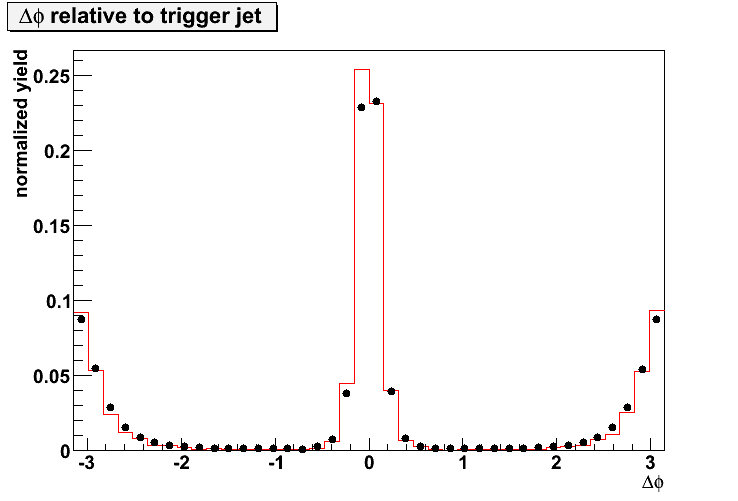
\includegraphics[width=0.7\textwidth]{figures/dphi}
  \caption{Azimuthal distribution of charged pions relative to the trigger jet axis in the 2006 dataset.  The black circles represent data, the red lines fully reconstructed Monte Carlo. Pions with $|\Delta \phi| > 2.0$ are accepted for analysis.}
  \label{fig:dphi}
\end{figure}

The data are binned as a function of \(z\), defined as the ratio of the
away-side pion \(p_T\) and the trigger jet \(p_T\). Figure~\ref{fig:meanpt}
shows that the jet \(\langle p_T \rangle\) is approximately constant as a
function of \(z\), and thus that the charged pion \(\langle p_T \rangle\)
increases linearly with \(z\). Again, the data are modeled well by STAR's
Pythia+GEANT simulations.

\begin{figure}
  \centering
  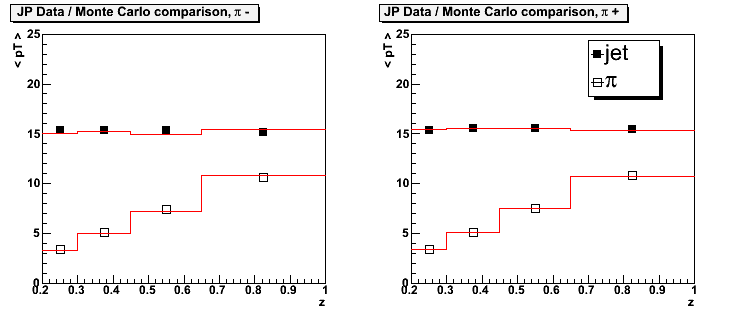
\includegraphics[width=1.0\textwidth]{figures/meanpt}
  \caption{Comparison of the $\langle p_T \rangle$ values for jets and charged pions in each $z$ bin.  The data show good agreement with fully reconstructed Pythia+GEANT events that pass a simulation of the BJP2 trigger.}
  \label{fig:meanpt}
\end{figure}

\section{Systematic Uncertainty Evaluations}
% beam polarization vectors and A_sigma - 1 day.  Don't go into too many details of the determination of the beam vector, just say it was based on an analysis of left/right and up/down asymmetries in the BBCs during longitudinal and transverse running.

\subsection{Polarization Vectors and Transverse Asymmetries}

The BBCs enable local polarimetry at STAR.  Vertical polarization in the beam generates an asymmetry in the counts recorded by the left and right halves of the BBC on which it impinges, while radial polarization generates an asymmetry in the top and bottom halves of the detector.  An accurate accounting of residual non-longitudinal polarization in the beams is important, because a double transverse spin asymmetry \(A_{\Sigma}\) could generate a false \(A_{LL}\).  The size of this false signal is given by the equation
%
\begin{equation}
  \delta A_{LL}^{\mathrm{non-longitudinal}} = | \tan(\theta_B) \tan(\theta_Y) \cos(\phi_B - \phi_Y) A_{\Sigma} |.
  \label{eqn:pol-vector-uncertainty}
\end{equation}
%
The beam polarization angles at STAR are determined through an analysis of cross ratios in the BBCs \cite{Kiryluk:2005gg}.  These ratios are directly sensitive to the azimuthal angle of the beam, and a comparison of the ratios in longitudinal and transverse running allows an extraction of the angle of inclination.  The measured ratio is 
%
\begin{equation}
  \epsilon_{BBC} = \frac{r_{ij} -1}{r_{ij} + 1} \simeq \left\{
  \begin{array}{l l}
    A_N^{BBC} \times P_v \times \langle \cos \phi \rangle & i,j = \mbox{Left, Right} \\
    A_N^{BBC} \times P_r \times \langle \sin \phi \rangle & i,j = \mbox{Up, Down} \\
  \end{array} \right.
\end{equation}
%
in which \(r_{ij} = \sqrt{\frac{N_i^{\uparrow} N_j^{\downarrow}}{N_i^{\downarrow} N_j^{\uparrow}}}\) and \(N_{i(j)}^{\uparrow(\downarrow)}\) are the spin dependent yields on the Left(Right) or Up(Down) side of the detector. \(P_{v(r)}\) is the vertical (radial) beam polarization.  Table~\ref{tab:pol-vectors} tabulates the extracted polarization vectors from measurements of the BBC cross-ratios.  There are two separate extractions for the 2006 data because the spin rotator magnets were adjusted midway through the run.  The data show a steady improvement in the performance of the spin rotators.

% due to the large non-statistical variations, ∼1.5 degrees, in the estimate of the polar angle coming from the the up/down asymmetries in the transverse running, we decided to use a conservative estimate of cos(φY − φB) = 1.

% that doesn't make much sense ... UD transverse asymmetries don't contribute to the determination of the polar angle to first order.

% also, the formulae to get the beam angles from these asymmetries are inconsistent.  But Murad's numbers for tan(theta) and phi do yield his numbers for the multiplicative factor in front of Asigma

% Table of Beam Polarization Vectors
\begin{table}
  \begin{center}
    \begin{tabular}{l|c|c}
      Run Period & Blue ($\theta, \phi$) & Yellow ($\theta, \phi$) \\
      \hline
      2005 & (7.9, 74.0) & (17.2, 138.7) \\
      2006a (7132001-7138034) & (6.9, 87.7) & (10.0, 34.4) \\ 
      2006b (7138035-7156040) & (0.9, 69.3) & (3.9, -47.8)
    \end{tabular}
  \end{center}
  \caption{Beam polarization vectors as determined from an analysis of up-down and left-right asymmetries in the BBCs.  The spin rotators were adjusted midway through the second longitudinal running period in 2006.}
  \label{tab:pol-vectors}
\end{table}


% use cos(phi_B - phi_Y) = 1 as conservative estimate since polar angle measurements exhibit non-statistical fluctuations in 2006.

% asigma graphs for 2006, cleaned up

% limited transverse running in 2005, different trigger thresholds in 2006.  Not fair to calculate A_sigma in 2006 and use it for 2005.  Assume 10%, flat in pT.  Not sure if it's justified by any data analysis I've done.


\subsection{Jet Transverse Momentum Shift}

The asymmetries calculated using the 2006 RHIC data are plotted against the
ratio of the charged pion \(p_{T}\) and the ``true'' \(p_{T}\) of the away-side
jet, which incorporates a number of corrections to the actual measured jet
\(p_T\). Various factors bias this measured quantity, including pileup tracks in
the TPC, finite resolution effects, possible detector miscalibrations,
out-of-cone hadronization of fragmenting partons, and in-cone underlying event
effects. The pileup and finite energy resolution are detector effects which can
be corrected in the analysis, while the remaining sources of bias are best
accounted for using a systematic uncertainty.

\subsubsection{Jet $p_T$ Scale Corrections}

TPC pileup has a relatively small effect on the jet momentum in the 2006 run. An
event-mixing analysis using zerobias data concluded that pileup adds an average
of 50 MeV to each jet. The bin migration caused by the $\sim$ 25\% jet energy
resolution results in a much larger \(p_T\) bias. This effect is investigated by
running the jet reconstruction algorithm on final-state particles in the Pythia
record to generate a ``particle'' jet and comparing the \(p_{T}\) of that jet
with the \(p_{T}\) of the ``detector'' jet formed from the tracks and towers of
the full detector simulation. The comparison is repeated for a broad envelope of
calibration parameters, tracking efficiencies, and detector states in order to
account for a possible detector miscalibration.

The hadronization and underlying event biases are not accounted for in the above
analysis. Out-of-cone hadronization is subprocess-dependent, since quark jets
typically have a harder fragmentation profile than gluon jets, while the
underlying event effect is isotropic in \(\eta \times \phi\) space and largely
independent of jet \(p_T\). However, the two effects are closely connected in
the Pythia Monte Carlo simulations. The combined effect from these two sources
of bias was estimated by comparing jets at the ``fragmented parton'' level with
the particle jets described above. In simulations of fragmented parton jets the
underlying event and hadronization processes are turned off.

Figure~\ref{fig:jet-pt-shift} plots the size of the shift from detector jet
\(p_T\) to particle jet \(p_T\) in bins of detector \(p_T\). The error bars
represent statistical uncertainties on the size of the shift, while the square
brackets denote combined systematic uncertainties from the detector
miscalibration envelope and the hadronization and underlying event effects. The
solid line is a polynomial fit to the data points:
%
\begin{equation}
  \Delta p_T = 1.538 - 0.1561*p_T - 0.001691*p_T^2.
\end{equation}
%
This shift is applied to each accepted jet before calculating the fragmentation
variable ``z'' used in the 2006 asymmetry analysis.

\begin{figure}
  \centering
  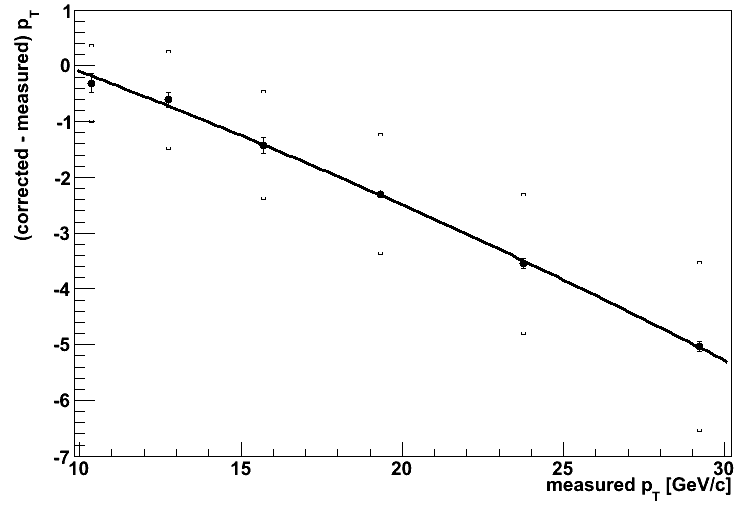
\includegraphics[width=0.7\textwidth]{figures/jet-pt-shift}
  \caption{Correction to measured jet $p_T$.  The data points represent the size of the shift in each measured jet $p_T$ bin, with statistical uncertainties attached.  The solid line is a polynomial fit to those data points, and the outer error bars represent systematic uncertainties due to detector miscalibration, out-of-cone hadronization, and underlying event effects summed in quadrature.}
  \label{fig:jet-pt-shift}
\end{figure}

\subsubsection{Effect on $A_{LL}$}

The bias on \(A_{LL}\) introduced by a systematic error in the jet \(p_T\) scale
corrections is estimated by a maximum extent uncertainty. We evaluate \(A_{LL}\)
using new \(p_T\) shift parameterizations generated from fits to the 1 $\sigma$
total uncertainty bands on the nominal \(p_T\) shift. The average magnitude of
the change in \(A_{LL}\) obtained using these alternative \(p_T\) shifts gives
us the size of the systematic uncertainty. The final values for this uncertainty
are given in Table~\ref{tab:syst-pt-shift}.

\begin{table}
  \centering
  \begin{tabular}{|c||c|c|}
    \hline
    $z$ & $\pi^-~\delta A_{LL}$ & $\pi^+~\delta A_{LL}$ \\
    \hline
    0.20 - 0.30 & 0.003 &  0.004 \\
    0.30 - 0.45 & 0.005 &  0.007 \\
    0.45 - 0.65 & 0.016 &  0.016 \\
    0.65 - 1.00 & 0.010 &  0.016 \\
    \hline
  \end{tabular}
  \caption{Systematic uncertainty on $A_{LL}$ due to possible errors in the correction from detector jet $p_T$ to true jet $p_T$.}
  \label{tab:syst-pt-shift}
\end{table}

\subsection{Trigger Bias}

STAR's BEMC jet patch trigger preferentially selects events where one of the
jets is located at mid-rapidity and hadronizes with a strong electromagnetic
component. This preference indirectly biases the triggered sample toward events
containing a quark jet, since quark jets have a harder fragmentation profile
than gluon jets. In addition, the jet that fires the trigger is unlikely to
contain a leading charged pion. The fragmentation bias in the trigger jet is a
primary reason that our analysis of the 2006 data is restricted to pions
opposite the trigger jet in azimuth.

The various biases introduced by the trigger are evaluated using a leading-order
Monte Carlo simulation of \(A_{LL}\) known as the Method of Asymmetry Weights.
Pythia supplies the kinematics and hard scattering subprocess of each simulated
event, which are sufficient to determine the partonic \(a_{LL}\) (calculated at
NLO in \cite{}). An ``asymmetry weight'' for the event is then constructed by
statistically sampling parton distribution functions:
%
\begin{equation}
  w = \frac{\Delta f_1(x_1, Q^2) * \Delta f_2(x_2, Q^2) * a_{LL}}{f_1(x_1, Q^2) * f_2(x_2, Q^2)},
\end{equation}
%
and one arrives at a Monte Carlo \(A_{LL}\) by simply taking the ratio of
asymmetry-weighted and unweighted distributions. The difference between the
\(A_{LL}\) for all Pythia events and the \(A_{LL}\) for reconstructed events
that satisfy a simulated trigger condition is used to assign the systematic
uncertainty.

\subsubsection{Monte Carlo Fragmentation Modeling}

The procedure described above requires that the Monte Carlo generator accurately
reproduces the real event kinematics. Unfortunately, the fragmentation tune in
Pythia~6 is not quite up to the task for STAR.
Figure~\ref{fig:subprocess-fractions} is a comparison of the subprocess
contributions to charged pion production reported by Pythia with the results of
NLO pQCD calculations incorporating Kretzer and DSS fragmentation functions. The
DSS set is known to better describe RHIC kinematics, but in
Figure~\ref{fig:subprocess-fractions} it's clear that Pythia agrees much better
with the Kretzer set.

\begin{figure}
  \subfloat[Kretzer]{
    \includegraphics[width=0.5\textwidth]{figures/pythia-kretzer}
    \label{fig:pythia-kretzer}
  }
  \subfloat[DSS]{
    \includegraphics[width=0.5\textwidth]{figures/pythia-dss}
    \label{fig:pythia-dss}
  }
  \caption{Comparison of subprocess contributions to charged pion production
  in Pythia and NLO pQCD calculations incorporating two different
  fragmentation functions.  The data points are results from Pythia and are the same in both plots. The Pythia results agree much better with the
  calculations using Kretzer fragmentation functions}
  \label{fig:subprocess-fractions}
\end{figure}

An accurate simulation of the subprocess contributions is an important
precondition for using the Method of Asymmetry Weights to evaluate trigger and
reconstruction bias, quite simply because $A_{LL}$ has such a strong subprocess
dependence. To confirm that the problem is really isolated to Pythia's
fragmentation functions, we examined the ratio of pions fragmenting from the
quark and the gluon in \(qg\) scattering events. That ratio is shown in Figure
\ref{fig:qg-fragmentation}, and confirms that the fragmentation model is
Kretzer-like, with much softer gluon fragmentation and/or harder quark
fragmentation than is observed at RHIC.

\begin{figure}
  \begin{center}
    \includegraphics[width=0.7\textwidth]{figures/qg-fragmentation}
  \end{center}
  \caption{Fraction of pions produced in quark-gluon scattering events that
  fragment from the gluon. Once again, the Pythia distributions agree much
  better with the calculation that uses Kretzer fragmentation functions.}
  \label{fig:qg-fragmentation}
\end{figure}

% the reweighting factor is the ratio of DSS and Kretzer FFs in each pT bin

% this reweighting factor is not applied in the 2006 analysis at the moment

Rather than plumb the depths of Pythia's independent fragmentation model, this
analysis applied a $p_{T}$- and subprocess-dependent reweighting factor to the
simulations to generate DSS-like fragmentation. The effect of this reweighting
is shown in Figure \ref{fig:compare-mcasym-nlo}. The filled markers show
markedly better agreement with the NLO pQCD calculations than the open markers,
particularly in scenarios such as GRSV-MIN where the difference in $A_{LL}$
between \(gg\) and \(qg\) subprocesses is large. The agreement is still not
perfect; one might speculate that Pythia gives too much weight to favored quark
fragmentation, since at high $p_{T}$ the $\pi^{-}$ asymmetries are too small
(indicating a relatively large d quark contribution) and the $\pi^{+}$
asymmetries are too large (consistent with a large u quark contribution).
However, as the trigger and reconstruction are not expected to be quark flavor
dependent we have decided to press forward with these simulations.

\subsubsection{2005 Bias Calculations}

\begin{figure}
  \includegraphics[width=\textwidth]{figures/compare-mcasym-nlo}
  \caption{Comparison of Monte Carlo asymmetries with NLO pQCD calculations
  incorporating DSS fragmentation functions. The open markers show results
  obtained using STAR's Pythia tune. The filled markers show the change in the
  asymmetries after reweighting the gg, qg, and qq distributions by the ratio
  of subprocess fractions calculated using DSS and Kretzer fragmentation
  functions.}
  \label{fig:compare-mcasym-nlo}
\end{figure}

Figure \ref{fig:mcasym-diff} examines the difference between asymmetries for a
``true'' sample using untriggered events and pions pulled straight from the
Pythia record, and a ``trigger+reco'' sample where the events must satisfy the
JP2 trigger simulator and the pion kinematics are obtained from TPC track
reconstruction. In some cases, the difference between the two samples is smaller
than the uncertainty on the ``trigger+reco'' sample (see Figure
\ref{fig:mcasym-sigma}). The systematic is assigned as the larger of the
difference in central values and the uncertainty on the ``trigger+reco'' sample.

The size of the systematic obviously depends on the polarized gluon
distributions that are included in the analysis. Previous measurements have
excluded the maximal polarization scenarios as well as scenarios with the
functional form of the GRSV set and integral gluon polarizations larger than 0.3
at \(Q^2 = 1 GeV^2\). As a result, we use an envelope defined by the GRSV M030
and P030 scenarios. The results of this analysis for the 2005 dataset are shown
in Table \ref{tbl:trig-reco-bias}.

% TODO recalculate bias systematic using M030 - P030 scenarios
% TODO better-looking plots for asymmetry difference and uncertainty

\begin{figure}
  \includegraphics[width=\textwidth]{figures/mcasym_run5_diff_rescaled}
  \caption{Difference between true and reconstructed Monte Carlo
  asymmetries after fragmentation reweighting.  The cyan and magenta curves represent polarized gluon distributions with the functional form of GRSV STD but with varying integral values for $\Delta G$.}
  \label{fig:mcasym-diff}
\end{figure}

\begin{figure}
  \includegraphics[width=\textwidth]{figures/mcasym_run5_sigma_rescaled}
  \caption{Uncertainty on reconstructed Monte Carlo asymmetries. If the
  uncertainty is larger than the difference between true and reconstructed
  asymmetries we use this to assign the systematic instead.}
  \label{fig:mcasym-sigma}
\end{figure}

\begin{table}[ht]
    \begin{center}
        \begin{tabular}{c|c|c}
        \hline
        $p_{T}$ & $\pi^{-}$ $\delta A_{LL}$ & $\pi^{+}$ $\delta A_{LL}$\\
        \hline
        2.00 - 3.18 & -0.0059 +0.0027 & -0.0061 +0.0061\\
        3.18 - 4.56 & -0.0083 +0.0072 & -0.0128 +0.0066\\
        4.56 - 6.32 & -0.0093 +0.0034 & -0.0176 +0.0101\\
        6.32 - 8.80 & -0.0072 +0.0036 & -0.0209 +0.0186\\
        8.80 - 12.84 & -0.0048 +0.0057 & -0.0152 +0.0062\\
    \hline
    \end{tabular}
    \end{center}
    \caption{2005 Trigger and Reconstruction Bias Uncertainties}
    \label{tbl:trig-reco-bias}
\end{table}

\subsubsection{2006 Bias Calculations}

An additional complication for the 2006 data analysis is shown in
Figure~\ref{fig:mean-pt-simu}. The JP trigger efficiency is a sharply-rising
function of jet \(p_T\); as a result, the \(\langle p_T \rangle\) for pions and
especially for jets in a given \(z\) bin is significantly larger in the
triggered sample compared to the minimum-bias sample. In effect, we are
under-sampling the low \(x\) regime in each \(z\) bin. The bias calculated by a
na\"ive application of the Method of Asymmetry Weights to this measurement would
be unacceptably large. Instead, we choose to publish the trigger efficiency as
part of the measurement, and to rescale the minimum-bias Monte Carlo sample by
that trigger efficiency. A comparison of the simulated \(A_{LL}\) in the
triggered and rescaled minimum-bias samples allows an estimate of the
measurement error introduced by the trigger's subprocess bias.

\begin{figure}
  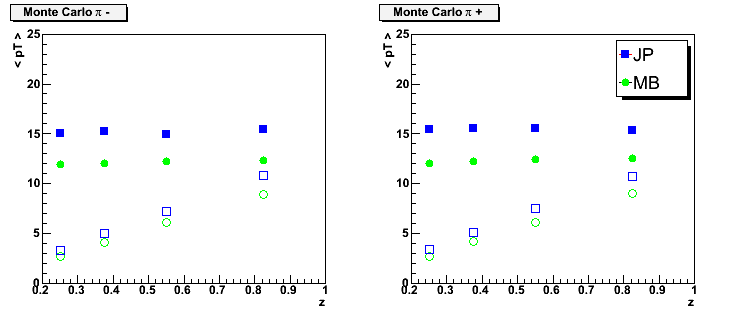
\includegraphics[width=1.0\textwidth]{figures/meanpt-by-trigger}
  \caption{Comparison of the $\langle p_T \rangle$ for MB and JP triggers ni the 2006 Monte Carlo.  Filled markers plot jet $\langle p_T \rangle$ and open markers charged pion $\langle p_T \rangle$. The JP triggered data sample has a dramatically larger jet $\langle p_T \rangle$ in each $z$ bin, which biases $A_{LL}$ towards larger values in the GRSV framework.}
  \label{fig:mean-pt-simu}
\end{figure}

Figure~\ref{fig:trigger-efficiency} plots the ratio of jet yields in the MB
Monte Carlo sample and the sample that passes a simulated JP trigger. The
trigger efficiency as a function of jet \(p_T\) is well described by a cubic
polynomial:
%
\begin{equation}
  \epsilon_{trigger} = 1.149 - 0.2655 * p_T   + 0.01857 * p_T^2 - 0.0003445 * p_T^3.
  \label{eqn:trigger-efficiency}
\end{equation}
%
Finally, Figure~\ref{fig:trig-bias-2006} plots the difference between the
trigger sample \(A_{LL}\) and the \(A_{LL}\) calculated from the rescaled MB
sample for an envelope of GRSV parameterizations with integral gluon
polarization less than 0.3 at \(Q^2 = 1 GeV^2\). A systematic uncertainty on our
measured \(A_{LL}\) is assigned by taking the maximum asymmetry difference in
each bin, or the uncertainty on the triggered \(A_{LL}\) if all asymmetry
differences are consistent with zero. The final values are tabulated in
Table~\ref{tab:trig-bias-2006}.

% TODO 2006 mcasym numbers for M030-P030
% TODO reweight 2006 Monte Carlo by DSS/Kretzer ratio

\begin{figure}
  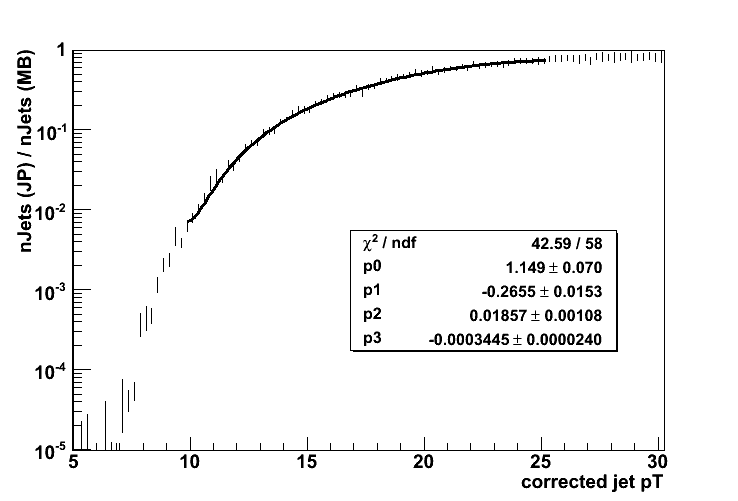
\includegraphics[width=1.0\textwidth]{figures/trigger-efficiency}
  \caption{A parameterization of the BJP1 trigger efficiency as a function of corrected jet $p_T$ established from the 2006 Monte Carlo.  This parameterization is used to factor out the trigger efficiency from the Method of Asymmetry Weights $A_{LL}$ studies, allowing those studies to focus on the subprocess bias inherent in the trigger.}
  \label{fig:trigger-efficiency}
\end{figure}

\begin{figure}
  \centering
  \includegraphics[width=0.5\textwidth]{figures/placeholder}
  \caption{Comparison of simulated asymmetries for triggered events and minimum-bias events which have been rescaled to reflect the average trigger efficiency as a function of jet $p_T$. The resulting difference is a measure of the bias introduced by the subprocess-dependence in the trigger.}
  \label{fig:trig-bias-2006}
\end{figure}

\begin{table}[ht]
    \begin{center}
        \begin{tabular}{c|c|c}
        \hline
        $z$ & $\pi^{-}$ $\delta A_{LL}$ & $\pi^{+}$ $\delta A_{LL}$\\
        \hline
        0.20 - 0.30 & 0.0 &  0.0 \\
        0.30 - 0.45 & 0.0 &  0.0 \\
        0.45 - 0.65 & 0.0 &  0.0 \\
        0.65 - 1.00 & 0.0 &  0.0 \\
    \hline
    \end{tabular}
    \end{center}
    \caption{2006 Trigger and Reconstruction Bias Uncertainties}
    \label{tab:trig-bias-2006}
\end{table}



% \subsection{Polarization Vectors and Transverse Asymmetries}

% data selection - 1/2 day

% pion identification - 1 day

% jet reconstruction - 1 day

% jet/pion correlations - 1/2 day.  Just a plot of the dphi matching in data and simulation ought to be enough.

% Systematic Uncertanties

% nothing for PID, but will i need to redo the run 6 analysis to subtract backgrounds? yes.  Can I assume nSigmaPion does not need to be recalibrated? probably - 4 days

% 2006 trigger bias includes the minbias Monte Carlo reweighting hackery - 2 days

% but not just the reweighting hackery, there's also an uncertainty in the size of the jet pT shift - 1 day.  And why don't I include pion pt shifts in that calculation?  Is it because I choose bin widths to match the pion pT resolution?

% Results - 1 day

% Conclusions - 1.5 days

% Cleanup - 2 days

\chapter{Results and Discussion}

We have reviewed the rich history of hadronic spin physics and
identified the need to more precisely constrain the polarized gluon
distribution. We described the experimental apparatus and the analysis
techniques used to collect and study millions of polarized proton collisions
towards that end. This chapter presents the final results of the analysis, a set
of asymmetries that are directly sensitive to polarized glue and allow a deeper
understanding of the fundamental nature of QCD in the nucleon.

\section{$A_{LL}$ for Inclusive Charged Pion Production}

Figure~\ref{fig:final-result-run5} presents the first measurement of \(A_{LL}\)
for inclusive charged pion production at the STAR experiment. The data are
plotted versus the \(p_T\) of the pion and are compared to a variety of NLO pQCD
predictions. The dashed black curve represents a prediction for \(A_{LL}\) based
on the GRSV Standard parameterization of \(\Delta g(x)\), which was derived in
2001 from a global fit to polarized DIS data. The MIN and ZERO curves correspond
respectively to maximally negative and zero gluon polarization in the nucleon.
Not shown is the fourth member of the GRSV set, corresponding to maximal gluon
polarization, which has been excluded by earlier measurements of \(A_{LL}\) in
other final-state channels (and is similarly excluded by this measurement).

The dashed magenta curve labeled GS Set C is based on a polarized gluon
distribution by Gehrmann and Stirling that has a small integral polarization in
the \(x\) range accessible to 200 GeV mid-rapidity measurements at RHIC, but in
fact has a very large polarization content at smaller values of \(x\). Future
correlation measurements and measurements at a 500 GeV center-of-mass energy
will enable STAR to test whether distribution functions of this form might
correspond to reality. Finally, the solid black curve represents a new
parameterization of \(\Delta g(x)\) by de Florian, Sassot, Stratmann, and
Vogelsang which is based on a global fit incorporating both DIS data and early
\(A_{LL}\) results from RHIC.\footnote{The measurements in this thesis are not
included in the current DSSV global fit.}

\begin{figure}[ht]
  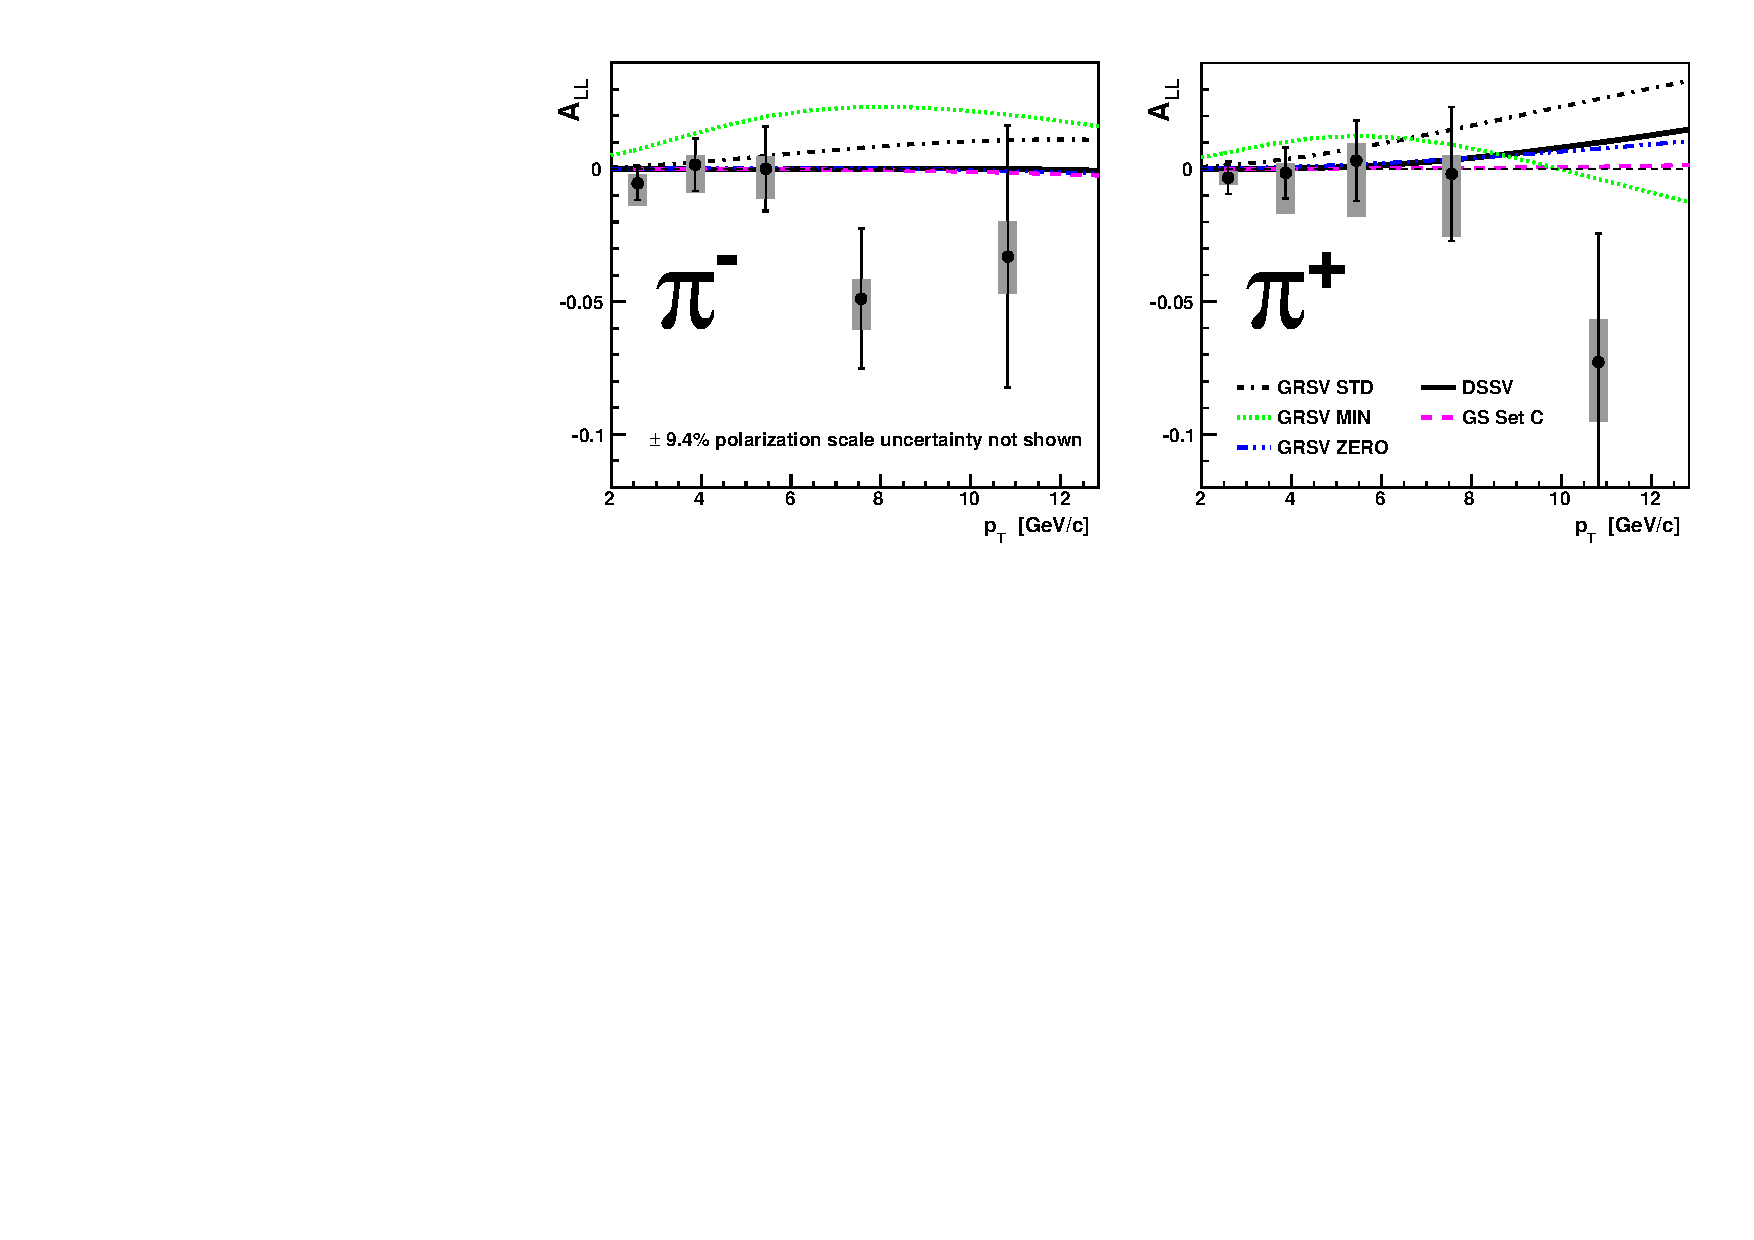
\includegraphics[width=1.0\textwidth]{figures/final-result-run5-2}
  \caption{$A_{LL}$ for inclusive charged pion production as a function of pion $p_T$ obtained from the 2005 dataset.  The error bars represent statistical uncertainties while the gray bands display total point-to-point systematic uncertainties.  The data are compared to NLO pQCD predictions incorporating various models for $\Delta g(x)$ \cite{Gluck:2000dy, Gehrmann:1995ag, deFlorian:2008mr}.}
  \label{fig:final-result-run5}
\end{figure}

\section{$A_{LL}$ for Jet + Pion Correlations}

Shown in Figure~\ref{fig:final-result-run6} are STAR's first measurements of
\(A_{LL}\) for charged pions opposite a trigger jet. The data are plotted versus
the fragmentation variable \(z\), using the away-side trigger jet \(p_T\) as a
surrogate for the \(p_T\) of the parton from which the pion fragmented. NLO pQCD
predictions for the measurement are plotted assuming the GRSV Standard, GS Set
C, and DSSV gluon distributions discussed above. The large difference in the
predictions for \(\pi^-\) \(A_{LL}\) and \(\pi^+\) \(A_{LL}\) at high \(z\) is a
reflection of the importance of favored fragmentation in that regime. Recall
that the \(\Delta u(x)\) distribution in the proton is uniformly positive, while
the \(\Delta d(x)\) distribution is smaller and uniformly negative. At high
\(z\), where the disparity between favored and disfavored fragmentation is
large, the \(\pi^-\) \(A_{LL}\) is driven by \(d\) quark scattering and the
\(\pi^+\) by \(u\) quark scattering. Favored fragmentation is also responsible
for the very different functional forms of the MIN \(A_{LL}\) prediction for
inclusive \(\pi^-\) and \(\pi^+\) \(A_{LL}\) in
Figure~\ref{fig:final-result-run5}.

\begin{figure}[]
  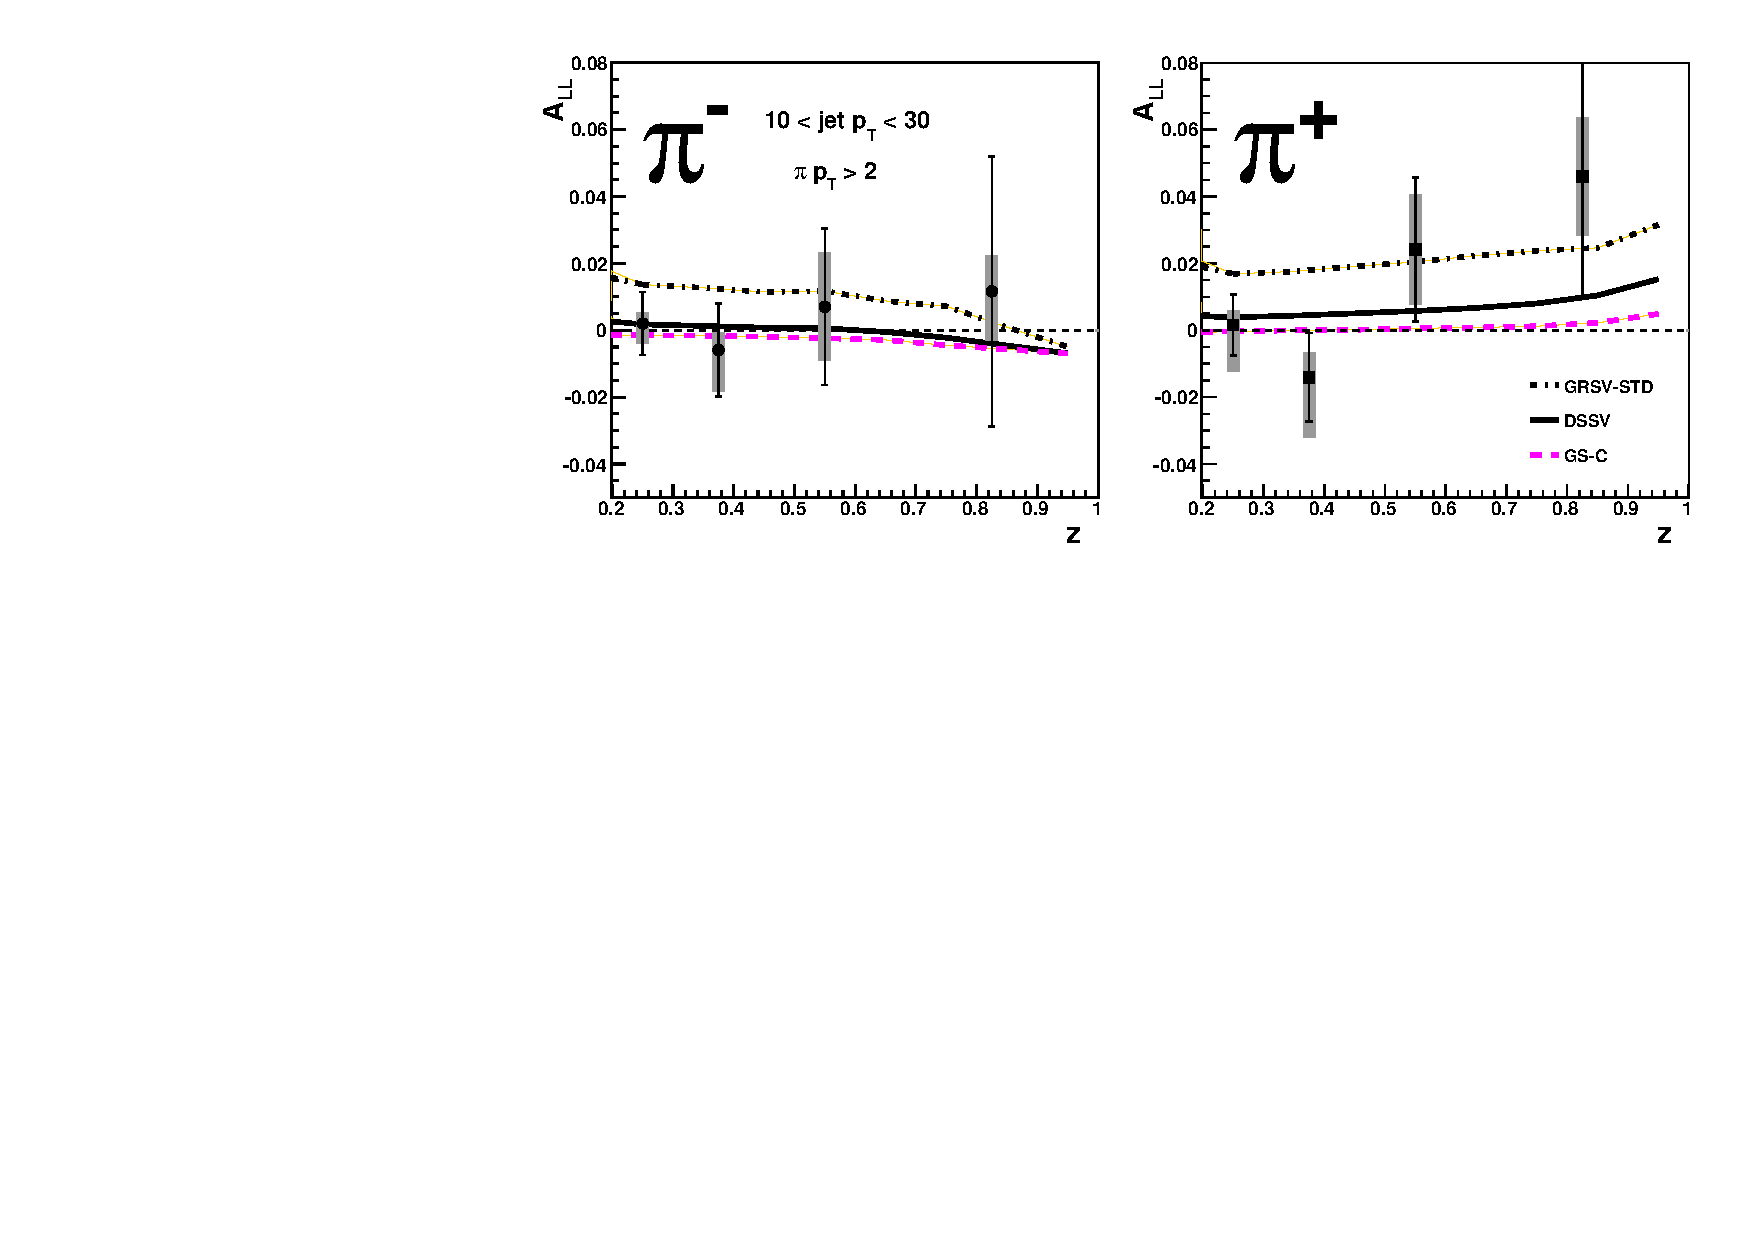
\includegraphics[width=1.0\textwidth]{figures/final-result-run6-4}
  \caption{$A_{LL}$ for charged pion production opposite an identified jet from the 2006 dataset.  The data are plotted against the ratio of the pion and jet transverse momenta, here labeled using the fragmentation variable $z$.  As in Figure~\ref{fig:final-result-run5}, the error bars represent statistical uncertainties and the gray bands point-to-point systematics.  The NLO predictions are the result of a recent analysis by de Florian \cite{deFlorian:2009fw}.}
  \label{fig:final-result-run6}
\end{figure}

\begin{table}
  \centering
  \begin{tabular}{|c||c|c|c||c|c|c|}
    \hline
    \multirow{2}{*}{$p_T$} & \multicolumn{3}{c||}{$\pi^{-}$} & \multicolumn{3}{c|}{$\pi^{+}$} \\
    \cline{2-7}
    & $A_{LL}$ & Stat. Error & Syst. Error &$A_{LL}$ & Stat. Error & Syst. Error\\
    (GeV/c) & ($10^{-3}$) & ($10^{-3}$) & ($10^{-3}$) & ($10^{-3}$) & ($10^{-3}$) & ($10^{-3}$) \\
    \hline
    \hline
    2.00 - 3.18 & -5.5 & $\pm$ 6.3 & -8.2 +3.4 &  -3.3 & $\pm$ 6.1 & -2.7 +2.2\\
    3.18 - 4.56 & 1.6 & $\pm$ 9.9 & -10.4 +3.4 &  -1.5 & $\pm$ 9.5 & -15.2 +3.5\\
    4.56 - 6.32 & 0.0 & $\pm$ 15.9 & -11.2 +4.6 &  3.1 & $\pm$ 15.2 & -21.1 +6.5\\
    6.32 - 8.80 & -48.9 & $\pm$ 26.4 & -11.4 +7.3 &  -1.9 & $\pm$ 25.2 & -23.5 +7.1\\
    8.80 - 12.84 & -33.0 & $\pm$ 49.4 & -14.0 +13.2 &  -72.8 & $\pm$ 48.5 & -22.2 +16.0\\
    \hline
  \end{tabular}
  \caption{$A_{LL}$ for inclusive charged pion production.}
  \label{tab:final-2005-result}
\end{table}

\begin{table}
  \centering
  \begin{tabular}{|c||c|c|c||c|c|c|}
    \hline
    \multirow{3}{*}{$z$} & \multicolumn{3}{c||}{$\pi^{-}$} & \multicolumn{3}{c|}{$\pi^{+}$} \\
    \cline{2-7}
    & $A_{LL}$ & Stat. Error & Syst. Error &$A_{LL}$ & Stat. Error & Syst. Error\\
    & ($10^{-3}$) & ($10^{-3}$) & ($10^{-3}$) & ($10^{-3}$) & ($10^{-3}$) & ($10^{-3}$) \\
    \hline
    \hline
    0.20 - 0.30 & 2.0 & $\pm$ 9.4 & -6.1 +3.2 &  1.6 & $\pm$ 9.1 & -14.0 +4.2\\
    0.30 - 0.45 & -5.9 & $\pm$ 13.9 & -12.4 +5.2 &  -14.1 & $\pm$ 13.2 & -18.0 +7.4\\
    0.45 - 0.65 & 7.0 & $\pm$ 23.4 & -16.1 +16.1 &  24.1 & $\pm$ 21.5 & -16.3 +16.5\\
    0.65 - 1.00 & 11.6 & $\pm$ 40.4 & -14.8 +10.6 &  46.0 & $\pm$ 36.5 & -17.7 +17.7\\
    \hline
  \end{tabular}
  \caption{$A_{LL}$ for charged pions opposite a trigger jet.}
  \label{tab:final-2006-result}
\end{table}

\section{Interpretation and Future Work}

A quantitive comparison of a measurement and an associated NLO prediction is obtained by calculating the \(\chi^2\) of the measurement with respect to the prediction.  One can then report the confidence level for that model of the polarized gluon distribution, which represents the probability that a \(\chi^2\) would exceed the observed \(\hat{\chi}^2\) if the model is correct.  Table~\ref{tab:confidence-levels} lists the confidence levels for all theoretical predictions plotted in Figures~\ref{fig:final-result-run5} and \ref{fig:final-result-run6}.  The \(\chi^2\) statistics are computed using statistical and point-to-point systematic uncertainties summed in quadrature.

The data are clearly incompatible with an assumption of maximally polarized gluons.  Maximally negative gluon polarization is also excluded at the 97.9\% level.  In general, the data are consistent with previous RHIC measurements in their preference for small values of gluon polarization.

The experimental methods described in this thesis are equally applicable to recent and future data taking at STAR.  A better understanding of systematic uncertainties in measurements of charged pion \(A_{LL}\) can be obtained through detailed Monte Carlo simulations of pion fragmentation as well as tighter constraints on the jet transverse momentum scale uncertainty.  Increases in luminosity and  polarization, as well as the first collisions at \(\sqrt{s} = 500\) GeV, speak to a bright future for RHIC as the experiments continue a comprehensive investigation into the spin structure of the nucleon.

\begin{table}
  \centering
  \begin{tabular}{|l||c|c|c|c|}
    \hline
    \multirow{2}{*}{Gluon Polarization Scenario} & \multicolumn{4}{c|}{Confidence Level} \\
    \cline{2-5}
    & 2005 $\pi^-$ & 2005 $\pi^+$ & 2006 $\pi^-$ & 2006 $\pi^+$ \\
    \hline
    GRSV $\Delta g$ = g & 1.6e-06 & 2e-07 & - & - \\
    GRSV $\Delta g$ = -g & 0.016 & 0.32 & - & - \\
    GRSV $\Delta g$ = 0 & 0.52 & 0.72 & - & - \\
    GRSV STD & 0.31 & 0.41 & 0.56 & 0.13 \\
    GS Set C & 0.53 & 0.79 & 0.98 & 0.59 \\
    DSSV & 0.52 & 0.71 & 0.98 & 0.59 \\
    \hline
  \end{tabular}
  \caption{Confidence levels of fitting predictions for $A_{LL}$ based on various polarized gluon distributions to the measurements presented in this thesis.}
  \label{tab:confidence-levels}
\end{table}

\end{fmffile}
% \appendix
% \include{appendices/appa}
% \include{appendices/appb}
\begin{singlespace}
\bibliography{main}
\bibliographystyle{plain}
\end{singlespace}
\end{document}

